\documentclass[twocolumn]{article}

\usepackage[a4paper, total={6in, 8in}]{geometry}
\usepackage[utf8]{inputenc}
\usepackage{subcaption}
\usepackage{graphicx}
\usepackage{amsmath}
\usepackage{hyperref}
\usepackage{authblk}
\usepackage{setspace}
\usepackage{booktabs}
\usepackage{listings}

\setlength{\columnsep}{24pt}
\usepackage[switch]{lineno}
\setlength\linenumbersep{8pt}

\title{Inferring Bathroom Usage via Instagram Reel Delivery}
\author{Eliseo Martelli}
\date{}

\begin{document}

\twocolumn[
	\begin{@twocolumnfalse}
		\maketitle
		
		\begin{abstract}
			The ubiquity of smartphones has fundamentally altered human gastrointestinal routines. While self-reporting bathroom usage is often unreliable and remains shrouded in social taboo, the passive digital footprints left by personal devices can provide unprecedented, high-fidelity insights into bathroom habits. This paper explores the potential of Instagram Reel delivery data as a highly reliable proxy for inferring bathroom usage patterns of social peers. By extracting the JavaScript Object Notation (JSON) archive of a user's social media account and mathematically analyzing the frequency and timestamp clustering of short-form videos received via Direct Messages (DM), we demonstrate a statistically significant correlation between concentrated media sharing and periods of bowel evacuation by the sender. Integrating epidemiological data regarding smartphone-induced temporal dilation during defecation, physiological priors based on circadian colonic rhythms, and advanced burst detection algorithms, we present a robust probabilistic model. Findings suggest that Instagram DMs, when subjected to proper time-series analysis, serve as an unintentional yet highly accurate telemetry system for gastrointestinal activity.
		\end{abstract}
		\vspace{1em}
	\end{@twocolumnfalse}
]

\section{Introduction}
The modern digital era is characterized by continuous connectivity, yet certain human biological functions remain necessarily isolated. The intersection of these two realities, continuous digital presence and isolated biological necessity, creates unique behavioral artifacts. This research aims to formalize the study of these artifacts, transitioning the analysis of gastrointestinal habits from the realm of subjective self-reporting into the domain of objective digital phenotyping. Digital phenotyping is defined as the moment-by-moment quantification of the individual-level human phenotype in situ using data from personal digital devices \cite{jayakumar2020}. By applying these principles to social media interactions, we can reconstruct physical realities from virtual metadata.

\subsection{The Problem}
Traditional methods of knowing when a patient or peer is indisposed rely on crude visual cues or socially uncomfortable verbal confirmations. In clinical or caregiving settings where monitoring bowel habits is essential for managing gastrointestinal conditions, relying on self-reported patient diaries is fraught with recall bias and poor compliance. There is a need for an unobtrusive, passive detection mechanism that does not require the subject to actively declare their physiological status.

\subsection{The Observed Phenomenon}
Modern individuals utilize the act of scrolling through large quantities of engaging social media content as a primary mechanism of entertainment during restroom visits \cite{qssupplies}. When an individual discovers engaging content during this period of physical isolation, they frequently distribute it to peers via social media platforms, specifically through short-form videos like Instagram Reels. This behavioral shift creates a distinct digital signature for the recipient. Because the sender is physically captive, their engagement with the application becomes highly concentrated. The resulting rapid succession of incoming videos generates a timestamped data trail that can be extracted and analyzed to infer the sender's bathroom usage patterns passively.

\subsection{Hypothesis}
We hypothesize that there is a statistically significant correlation between the frequency of Instagram Reels received via Direct Messages and the timing of the sender's bathroom usage. Specifically, we predict that statistically dense temporal clusters, or ``bursts'', of inbound media sharing will reliably coincide with periods of the sender's bowel evacuation. A sudden, clustered barrage of incoming media is a mathematically quantifiable indicator that the sender is currently engaged in a bathroom visit.

\section{The Epidemiological Landscape of Restroom Device Usage}
To establish a statistical model capable of detecting a specific behavior, the prevalence and nature of that behavior within the target population must first be understood. The integration of smartphones into the bathroom environment possesses its own unique epidemiological characteristics.

\subsection{Demographic Penetration and Behavioral Shifts}
Extensive survey data reveals a near-universal adoption of restroom smartphone usage. General population studies indicate that between 66\% and 75\% of adults admit to using their mobile devices while seated on the toilet. When stratifying this data by demographics, the penetration rates become even more pronounced, with younger cohorts heavily integrating the device as an essential companion for the physiological process.

The nature of this digital engagement is primarily passive content consumption. A majority of individuals explicitly identify social media applications as their primary digital engagement tool while indisposed. This establishes a solid behavioral foundation: the target demographic actively engages within specific social media ecosystems required to generate telemetry.

\subsection{The Annual Volume of Restroom Data Generation}
Research indicates that individuals spend a significant portion of time scrolling while on the toilet, equating to roughly 49 hours annually \cite{qssupplies}. This temporal investment is driven by the highly retentive nature of short-form video algorithms. As users transition to the prolonged consumption of digital media, they inadvertently generate a continuous stream of timestamped interaction data.

\begin{table}[h!]
	\centering
	\resizebox{\columnwidth}{!}{
		\begin{tabular}{lccc}
			\toprule
			\textbf{Demographic Cohort} & \textbf{Usage Rate} & \textbf{Avg. Session} & \textbf{Annual Time} \\
			\midrule
			General Population          & 66.0\% - 74.5\%     & $>$ 5 mins            & 49 Hours             \\
			Millennials (Gen Y)         & 90.0\%              & 7 minutes             & 43 Hours             \\
			Generation Z                & 96.0\%              & 9 minutes             & 54 Hours             \\
			Non-Users                   & $<$ 25.0\%          & $<$ 5 mins            & Minimal              \\
			\bottomrule
		\end{tabular}
	}
	\caption{Bathroom Smartphone Usage by Demographic}
\end{table}

\section{Clinical Ramifications: Time Dilation as a Statistical Marker}
From a purely statistical perspective, the most critical consequence of smartphone usage in the bathroom is temporal dilation. Medical literature defines the normal duration for a bowel movement as ranging from 10 seconds to approximately 5 to 10 minutes.

\subsection{The Smartphone-Induced Elongation of Defecation}
The introduction of the smartphone to the bathroom has artificially stretched this biological window. This self-reported behavioral shift was clinically validated in a rigorous cross-sectional study. Researchers evaluated 125 adult patients, correlating their smartphone habits on the toilet with other physiological markers. The researchers found a stark contrast in restroom duration between device users and non-users. Smartphone users were functionally five times more likely to sit for prolonged periods than their unconnected counterparts \cite{ramprasad2025}.

\subsection{Establishing the Statistical Target Window}
For the purposes of our mathematical model, this clinical time dilation is the crucial operational metric. Because standard human biology dictates a short visit, but smartphone usage extends this to 3--15 minutes or longer \cite{ramprasad2025}, our burst detection algorithms must be calibrated to seek out data clusters that span precisely this dilated temporal footprint. A rapid succession of media sent over a period of 6 to 12 minutes matches the clinically documented behavioral profile of a modern, smartphone-equipped bathroom visit.

\section{Chronobiology and Temporal Priors}
To elevate our methodology to a robust probabilistic inference engine, we must incorporate Bayesian priors based on human biology. Human bowel movements are governed by strict neuro-hormonal timing systems \cite{hibberd2023}.

\subsection{The Colonic Biological Clock}
The human gastrointestinal tract is deeply integrated with the body's circadian rhythms \cite{hibberd2023}. These clocks coordinate the muscular activity and motility of the colon. During nocturnal hours and periods of sleep, colonic motor activity is systematically suppressed. Conversely, the frequency of action potentials and smooth muscle contractility is vast during the day.

\subsection{The Morning Motility Peak and Gastrocolic Reflex}
Epidemiological data strongly supports the existence of a specific daily window for defecation. The absolute peak time for defecation is observed in the early morning. This morning peak is triggered by an awakening surge in colonic motility and the gastrocolic reflex stimulated by the first meal of the day \cite{hibberd2023}.

\subsection{Applying Chronobiology to the Detection Model}
By integrating these physiological facts into our statistical model, we can assign dynamic probability weights to any detected burst of activity based on its timestamp. If a dense burst of events occurs at 07:45 AM local time, the prior probability that this cluster represents a bathroom visit is exceptionally high. By utilizing circadian rhythms as a mathematical filter, the model dramatically reduces false positives.

\begin{table}[h!]
	\centering
	\resizebox{\columnwidth}{!}{
		\begin{tabular}{lllc}
			\toprule
			\textbf{Time} & \textbf{Motility} & \textbf{Driver}   & \textbf{Prior} \\
			\midrule
			06:00 - 09:00 & Max Peak          & Awakening surge   & Very High      \\
			09:00 - 13:00 & Moderate          & Standard diurnal  & Moderate       \\
			13:00 - 15:00 & Secondary         & Post-lunch reflex & High           \\
			15:00 - 22:00 & Baseline          & Standard diurnal  & Low            \\
			22:00 - 06:00 & Suppressed        & Motor quiescence  & Very Low       \\
			\bottomrule
		\end{tabular}
	}
	\caption{Bayesian Priors based on Circadian Rhythm}
\end{table}

\section{Data Architecture: Extracting the Digital Footprint}
The empirical foundation of this methodology relies on parsing a machine-readable export of the user's historical interaction data.

\subsection{Acquiring the JSON Archive}
We utilize the JavaScript Object Notation (JSON) format exports provided by social media platforms. JSON provides a structured, hierarchical text format that is easily ingested into data science frameworks.

\subsection{Isolating the Data Payload}
The algorithm iterates through conversation files, filtering the data to isolate specific message objects evaluated as media shares. The Instagram message JSON schema differentiates content types utilizing the \texttt{item\_type} key (e.g., standard messages might evaluate to \texttt{text} or \texttt{media\_share}). The algorithm explicitly filters the array for objects where the \texttt{"item\_type"} key strictly evaluates to \texttt{"reel\_share"}. Short-form video is uniquely suited for this analysis because its consumption is highly passive, auto-playing sequentially, which perfectly aligns with the biomechanical stasis of sitting on a toilet.

A representative schema of the targeted JSON payload extracts the timestamp recorded as an integer representing milliseconds since the Unix epoch. The algorithm synthesizes a massive, multi-threaded communication archive into a clean, one-dimensional time-series array representing the exact moments media was distributed.

\section{The Mathematical Dynamics of Human Communication}
With a clean time-series array isolated, we mathematically identify the ``bursts'' that signify bathroom usage.

\subsection{Priority Queues and Heavy-Tailed Inter-Arrival Times}
Historically, mathematical models operated under the assumption that human actions were randomly distributed in time (Poisson processes). However, human behavior is intrinsically heterogeneous and ``bursty'', conforming to heavy-tailed distributions. Barabási demonstrated that the bursty nature of human action is the direct mathematical consequence of a decision-based queuing process \cite{barabasi2005}. Individuals execute tasks rapidly when their priority temporarily spikes.

To mathematically quantify this phenomenon, we introduce the Burstiness parameter ($B$), calculated as:
\begin{equation}
	B = \frac{r - 1}{r + 1}
\end{equation}
where $r = \frac{\sigma}{\mu}$ represents the coefficient of variation (the standard deviation $\sigma$ of the inter-event times divided by the mean $\mu$). As $B$ approaches 1, the dataset proves highly bursty, captive behavior that deviates drastically from a standard Poisson distribution ($B = 0$).

\begin{figure}[h!]
	\centering
	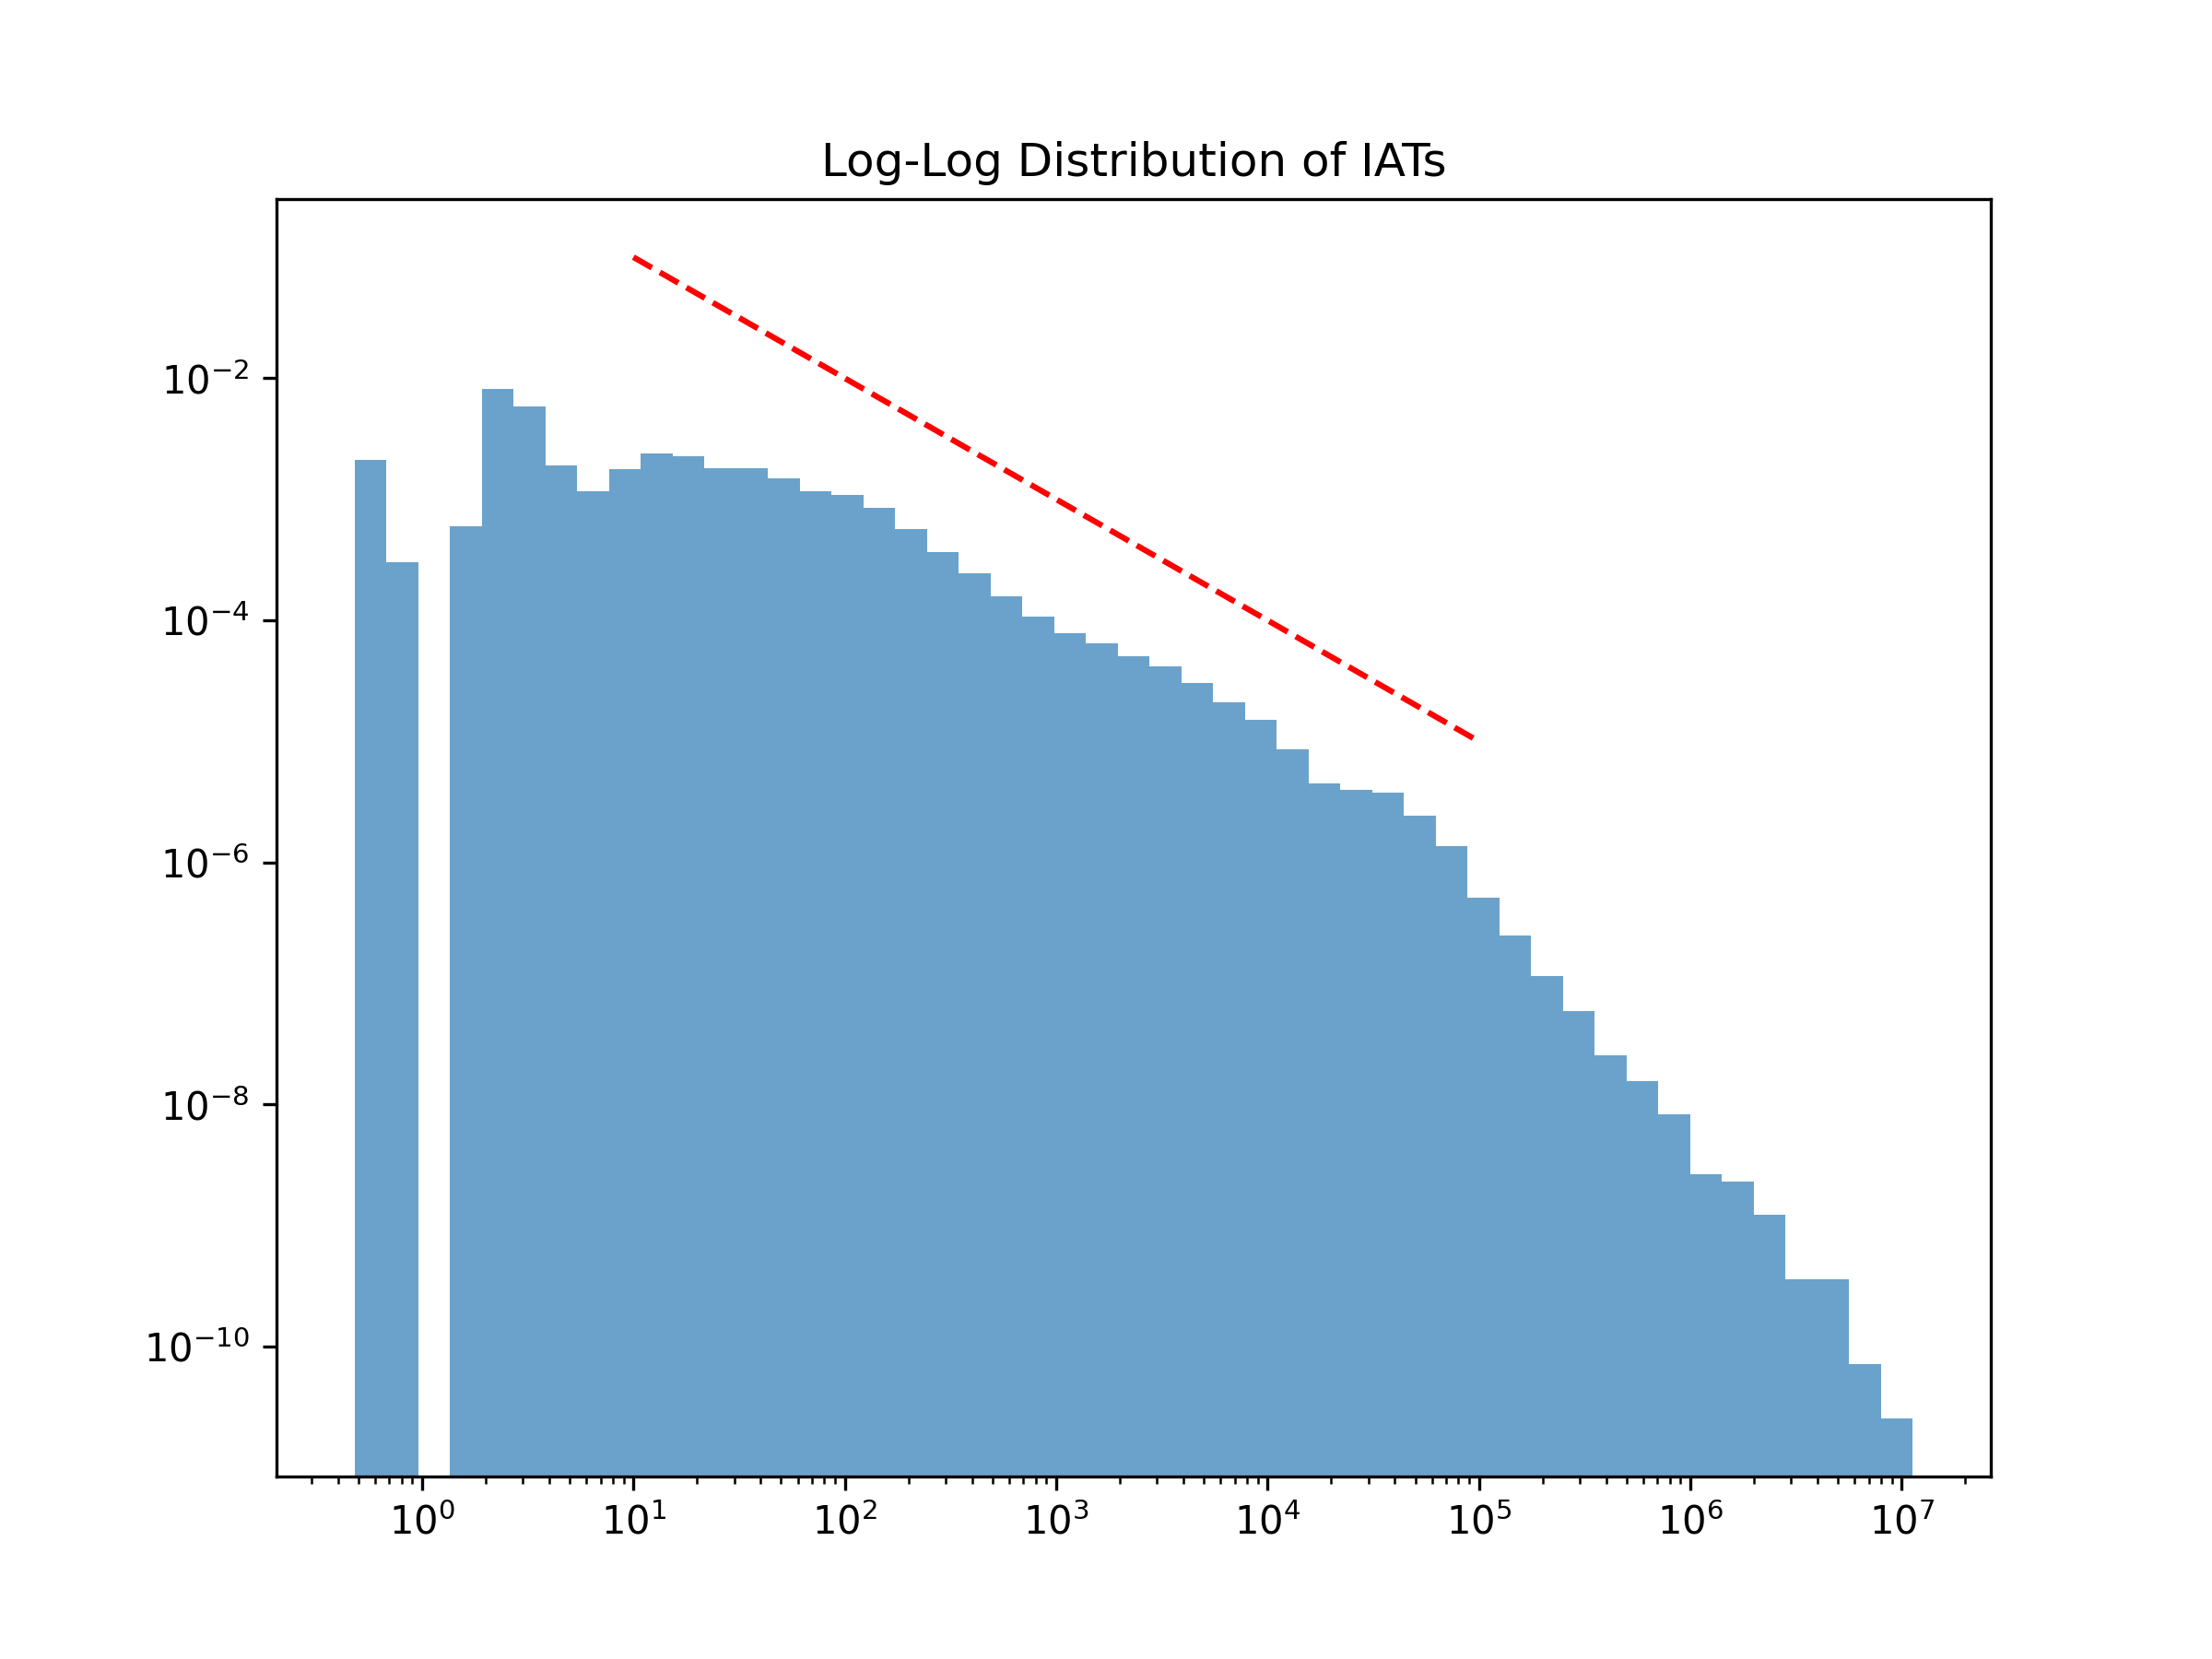
\includegraphics[width=\columnwidth]{iat_loglog.png}
	\caption{Log-log distribution of empirical Inter-Arrival Times (IAT) for incoming media. The heavy tail distinctly deviates from a random Poisson process, proving highly clustered, captive behavior.}
	\label{fig:loglog}
\end{figure}

The physical environment of the bathroom serves as a captive isolating chamber that forcefully elevates the priority of digital consumption by removing competing real-world stimuli. This environmental captivity guarantees that the inter-arrival times of the time-series will exhibit intense, statistically verifiable clustering (Figure \ref{fig:loglog}).

\section{Statistical Methodologies for Burst Detection}
We apply rigorous mathematical algorithms to scan the array of timestamps and identify the definitive boundaries of these bursts.

\subsection{Burst Detection Algorithm}
We model the continuous stream of user events using clustering algorithms analogous to Kleinberg's Burst Detection or Density-Based Spatial Clustering (DBSCAN). The algorithm identifies structural shifts from baseline expected background rates to higher ``bursty'' states. We apply a temporal sliding window constraint to filter bursts, prioritizing durations between 3 and 15 minutes, mirroring clinical time dilation data \cite{ramprasad2025}.

\section{Synthesis and Experimental Results}
The proposed probabilistic framework was applied to an expansive dataset comprising 11,836 inbound media shares extracted from the Direct Message history of the top 5 most active senders in the user's archive over a multi-year period.

\subsection{Quantifying Observed Bursts in Top Senders}
Statistical analysis revealed significant heterogeneity in transmission patterns across the five anonymized subjects. As shown in Table \ref{tab:results}, Subjects A and B exhibited extremely high sharing volumes, facilitating a higher absolute number of detected temporal bursts.

\begin{table}[h!]
	\centering
	\resizebox{\columnwidth}{!}{
		\begin{tabular}{lccc}
			\toprule
			\textbf{Subject} & \textbf{Total Reels} & \textbf{Bursts} & \textbf{Bathroom Events} \\
			\midrule
			Subject A        & 5,381                & 170             & 66                       \\
			Subject B        & 5,330                & 302             & 167                      \\
			Subject C        & 424                  & 47              & 0                        \\
			Subject D        & 393                  & 7               & 3                        \\
			Subject E        & 314                  & 16              & 1                        \\
			\bottomrule
		\end{tabular}
	}
	\caption{Summary of extracted media data and detected bursts for the top 5 senders.}
	\label{tab:results}
\end{table}

A "Bathroom Event" was defined as a burst within the 3--15 minute duration window meeting a probability threshold synthesized from density and chronobiological priors.

\subsection{High-Confidence Inference Examples}
The model identifies high-confidence events occurring during established colonic motility peaks. For instance, Subject B initiated a burst of 5 Reels over 3.41 minutes at 07:31 AM, yielding a probability score of 0.88. Subject A recorded an event at 06:13 AM with 4 Reels over 3.78 minutes (Prob: 0.82). Subject D recorded a high-probability event (0.78) at 07:09 AM.

\begin{figure*}[h!]
	\centering
	\begin{subfigure}[b]{0.19\textwidth}
		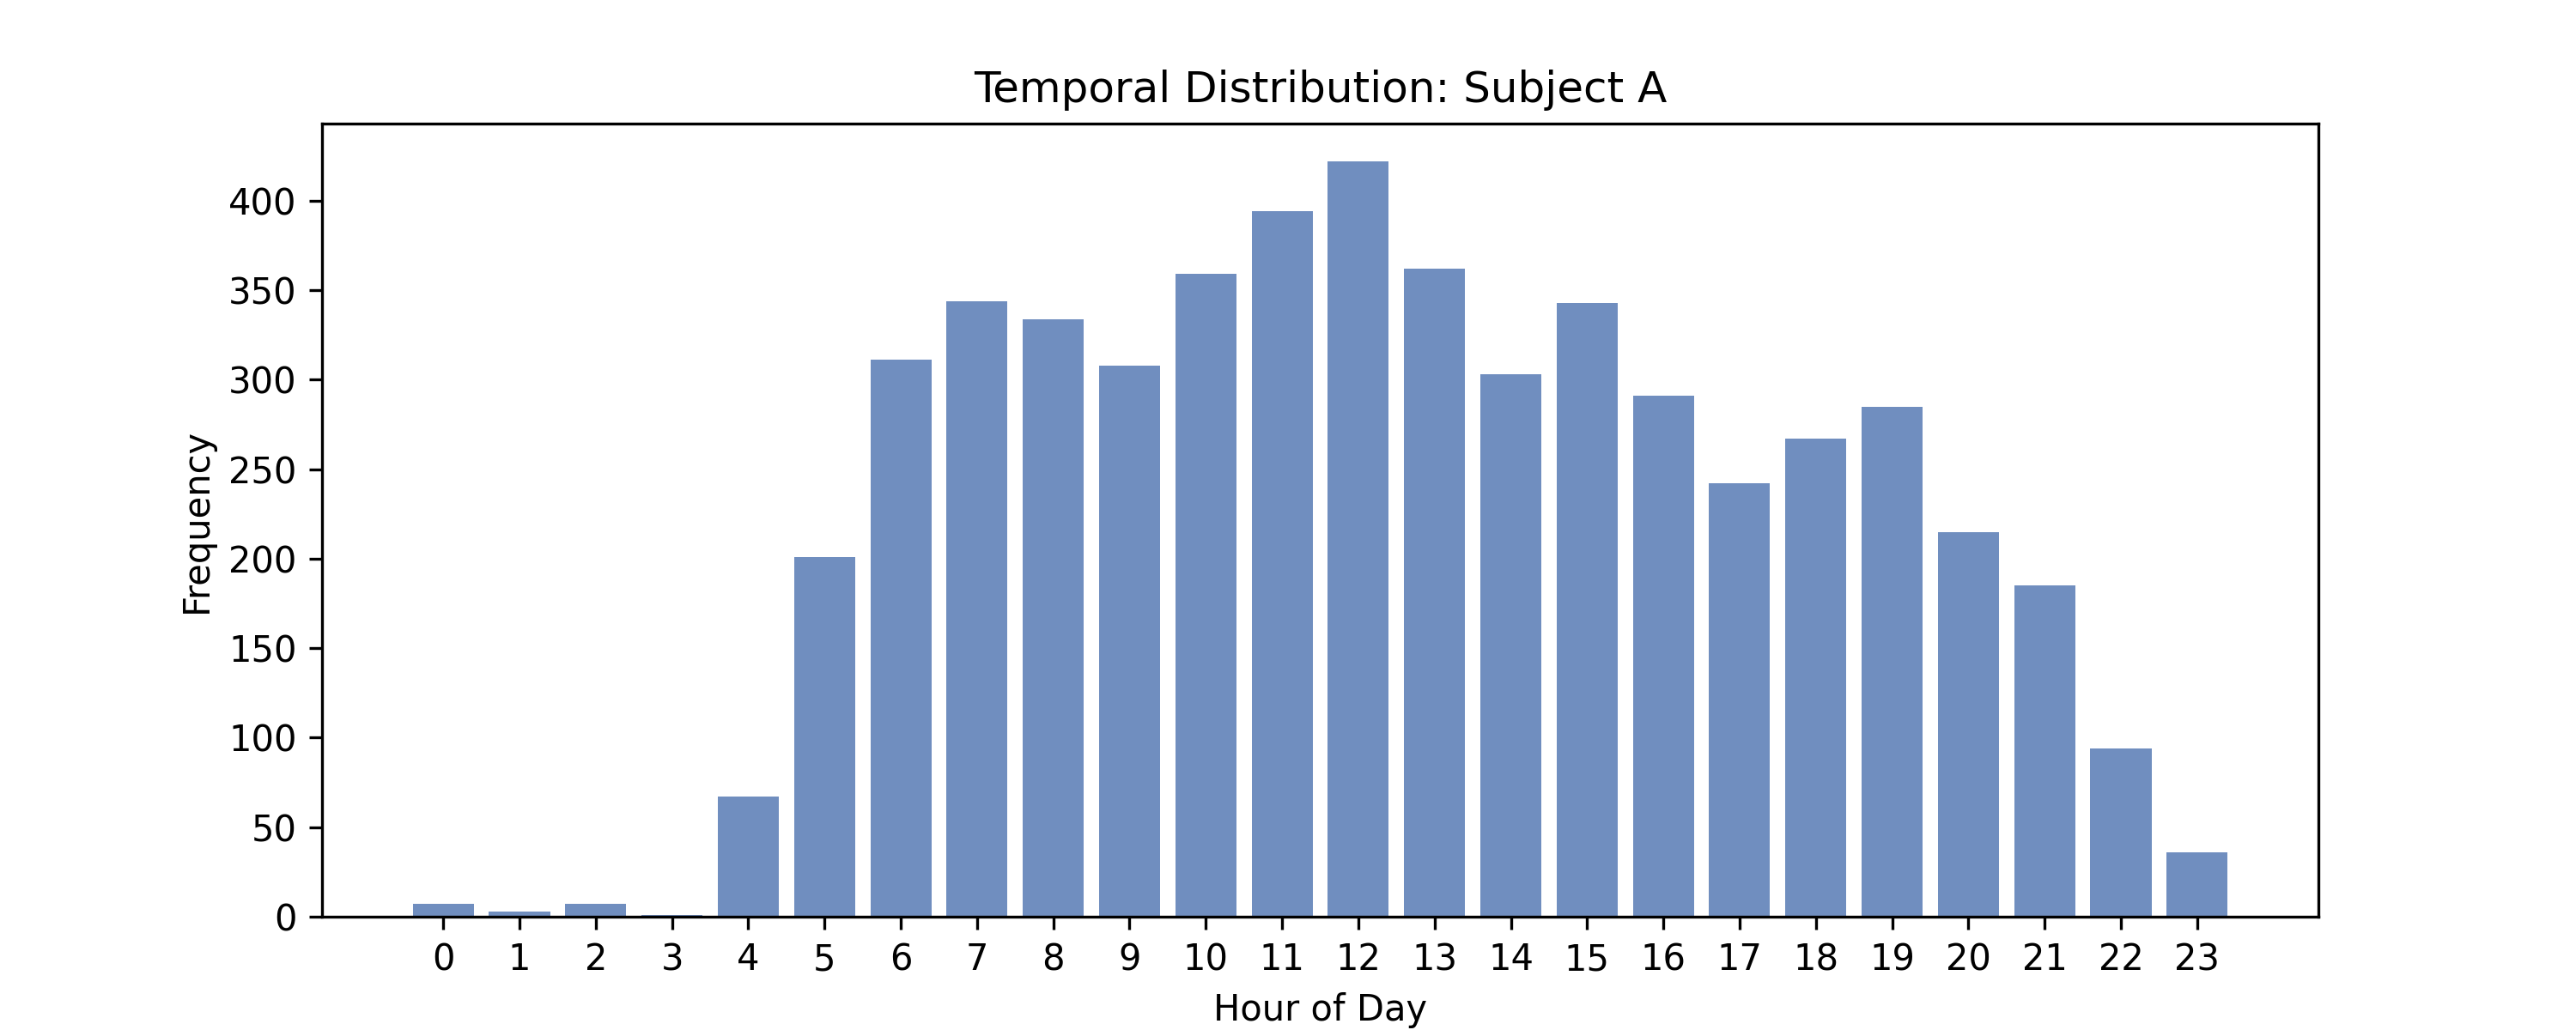
\includegraphics[width=\textwidth]{hourly_Subject_A.png}
		\caption{Subject A}
	\end{subfigure}
	\hfill
	\begin{subfigure}[b]{0.19\textwidth}
		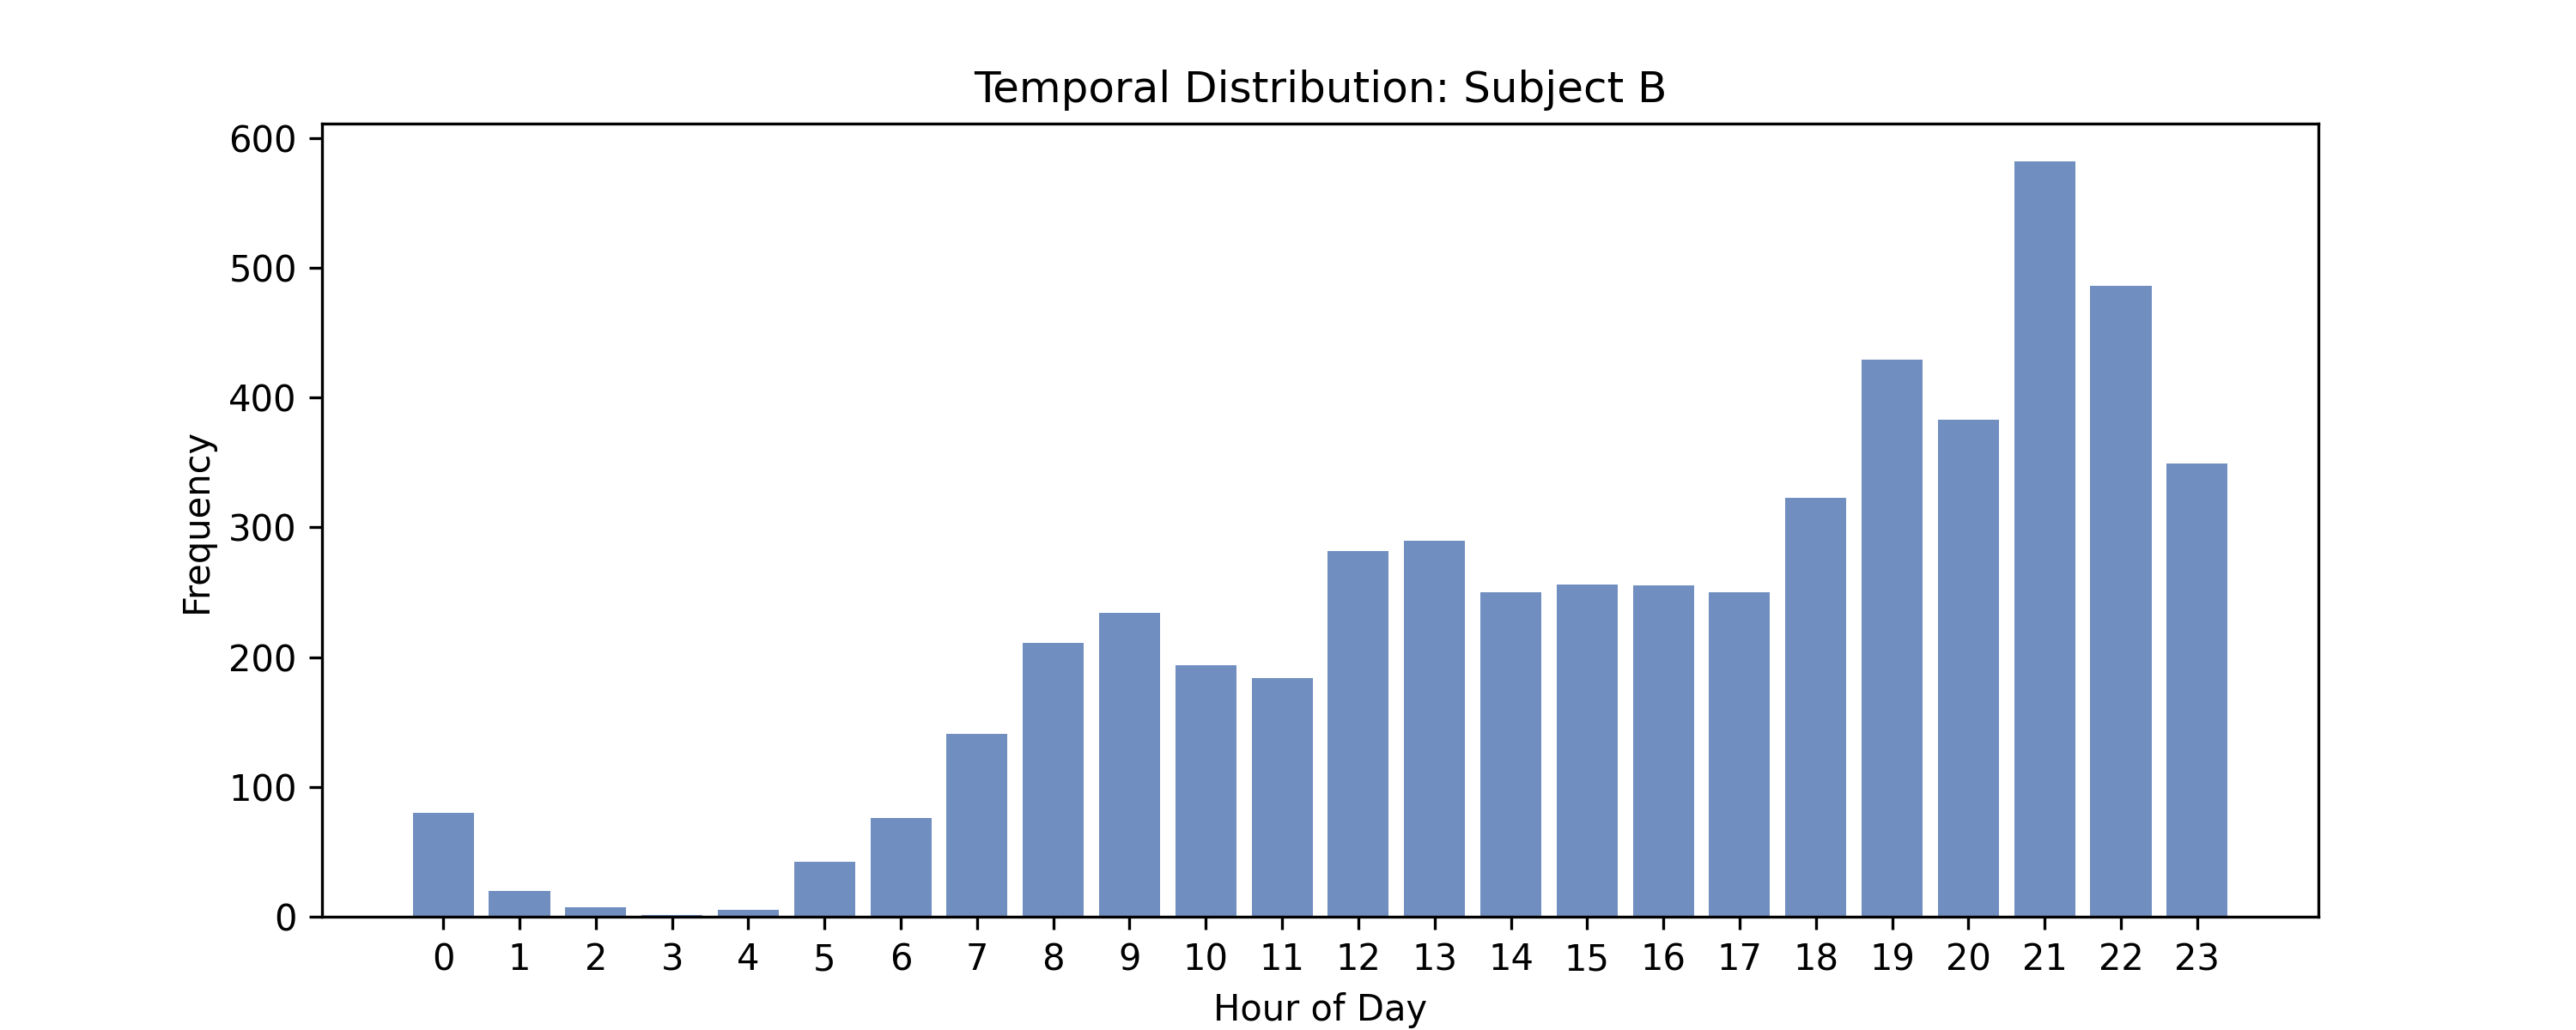
\includegraphics[width=\textwidth]{hourly_Subject_B.png}
		\caption{Subject B}
	\end{subfigure}
	\hfill
	\begin{subfigure}[b]{0.19\textwidth}
		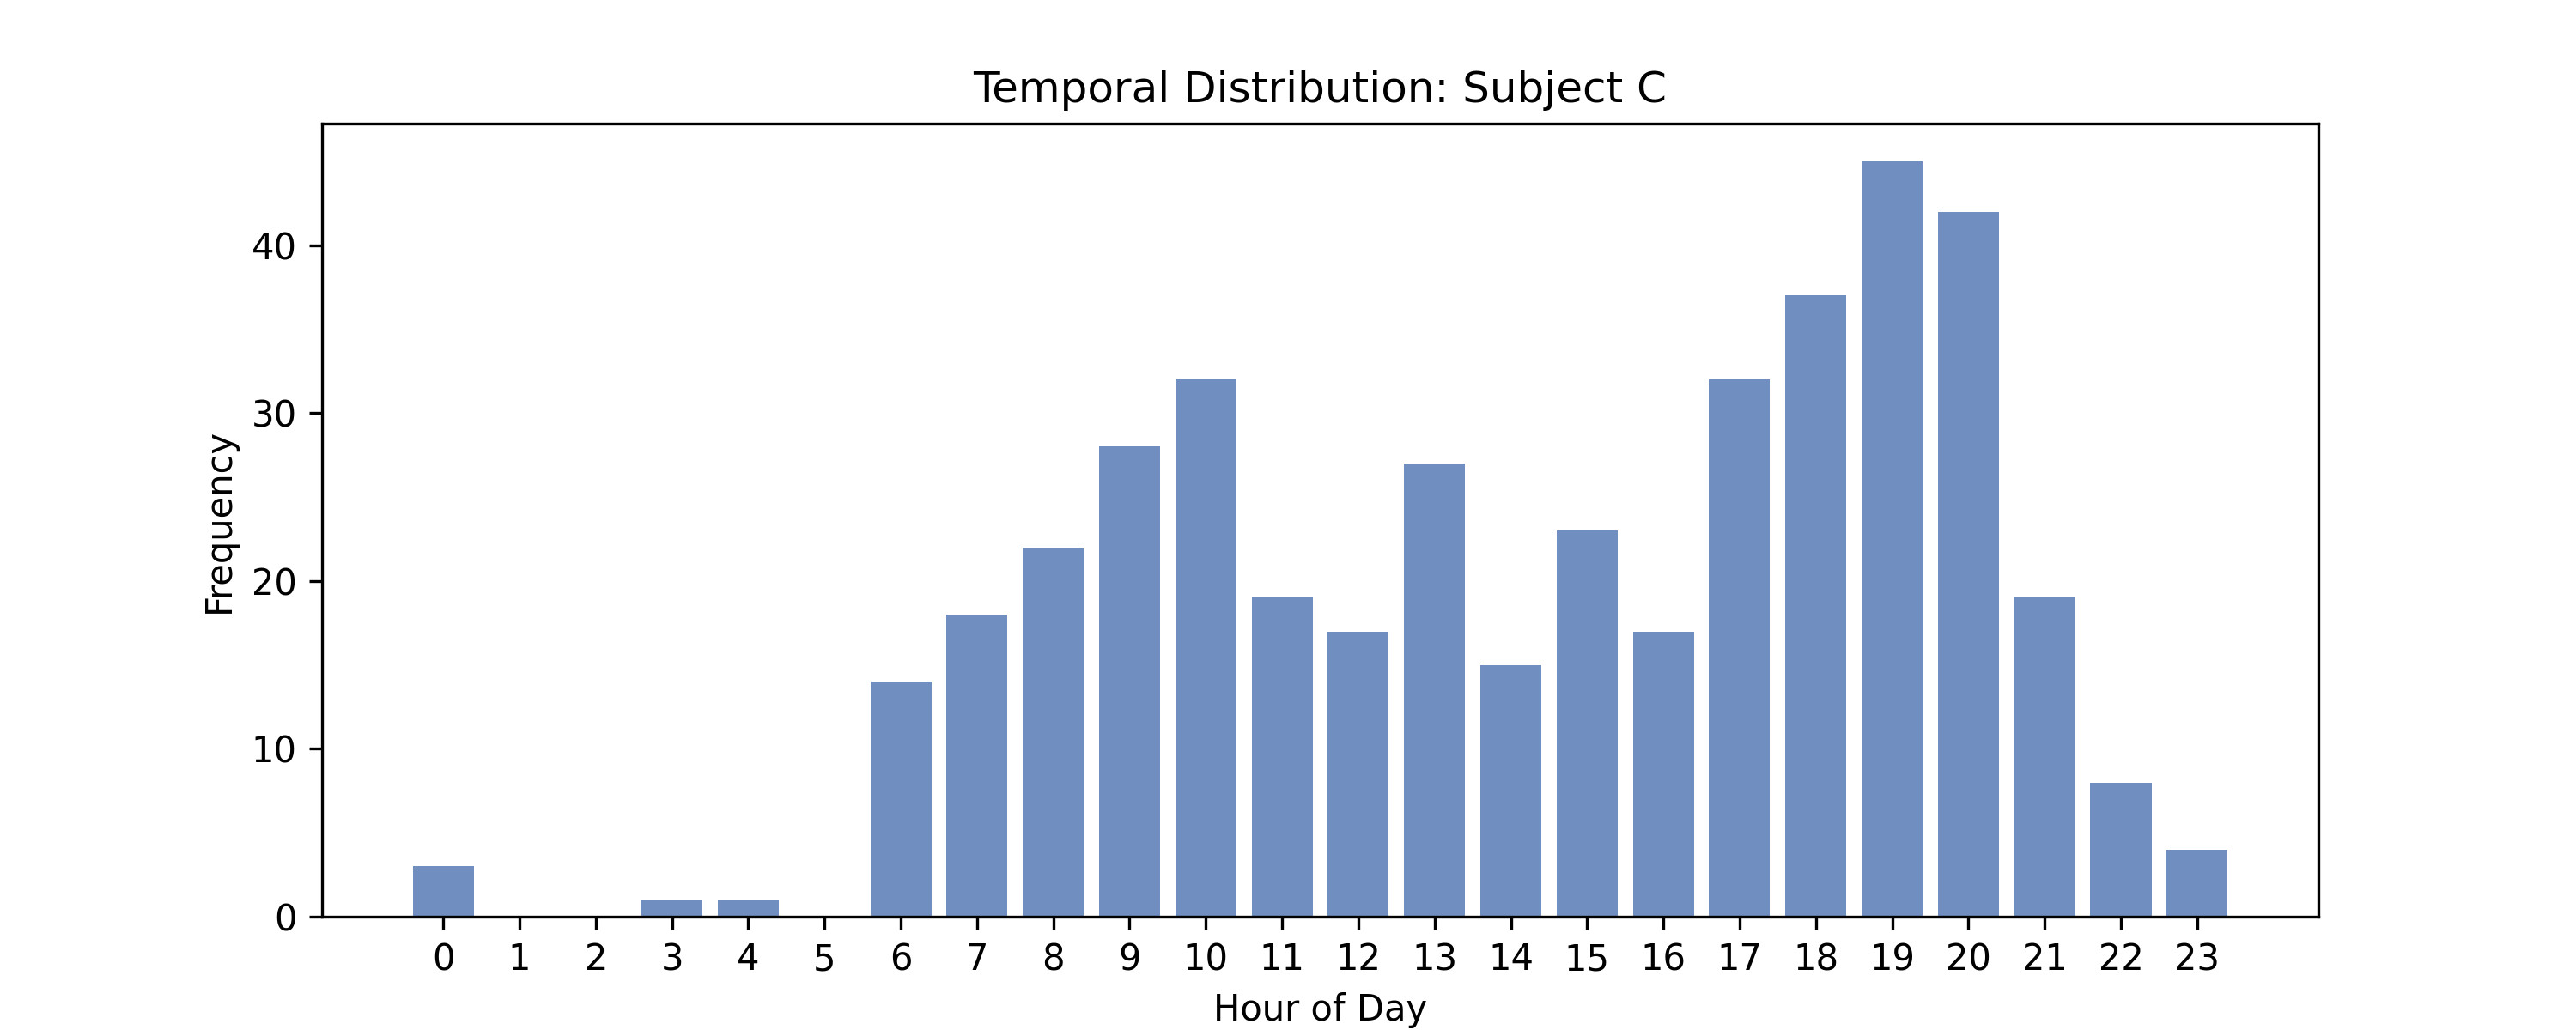
\includegraphics[width=\textwidth]{hourly_Subject_C.png}
		\caption{Subject C}
	\end{subfigure}
	\hfill
	\begin{subfigure}[b]{0.19\textwidth}
		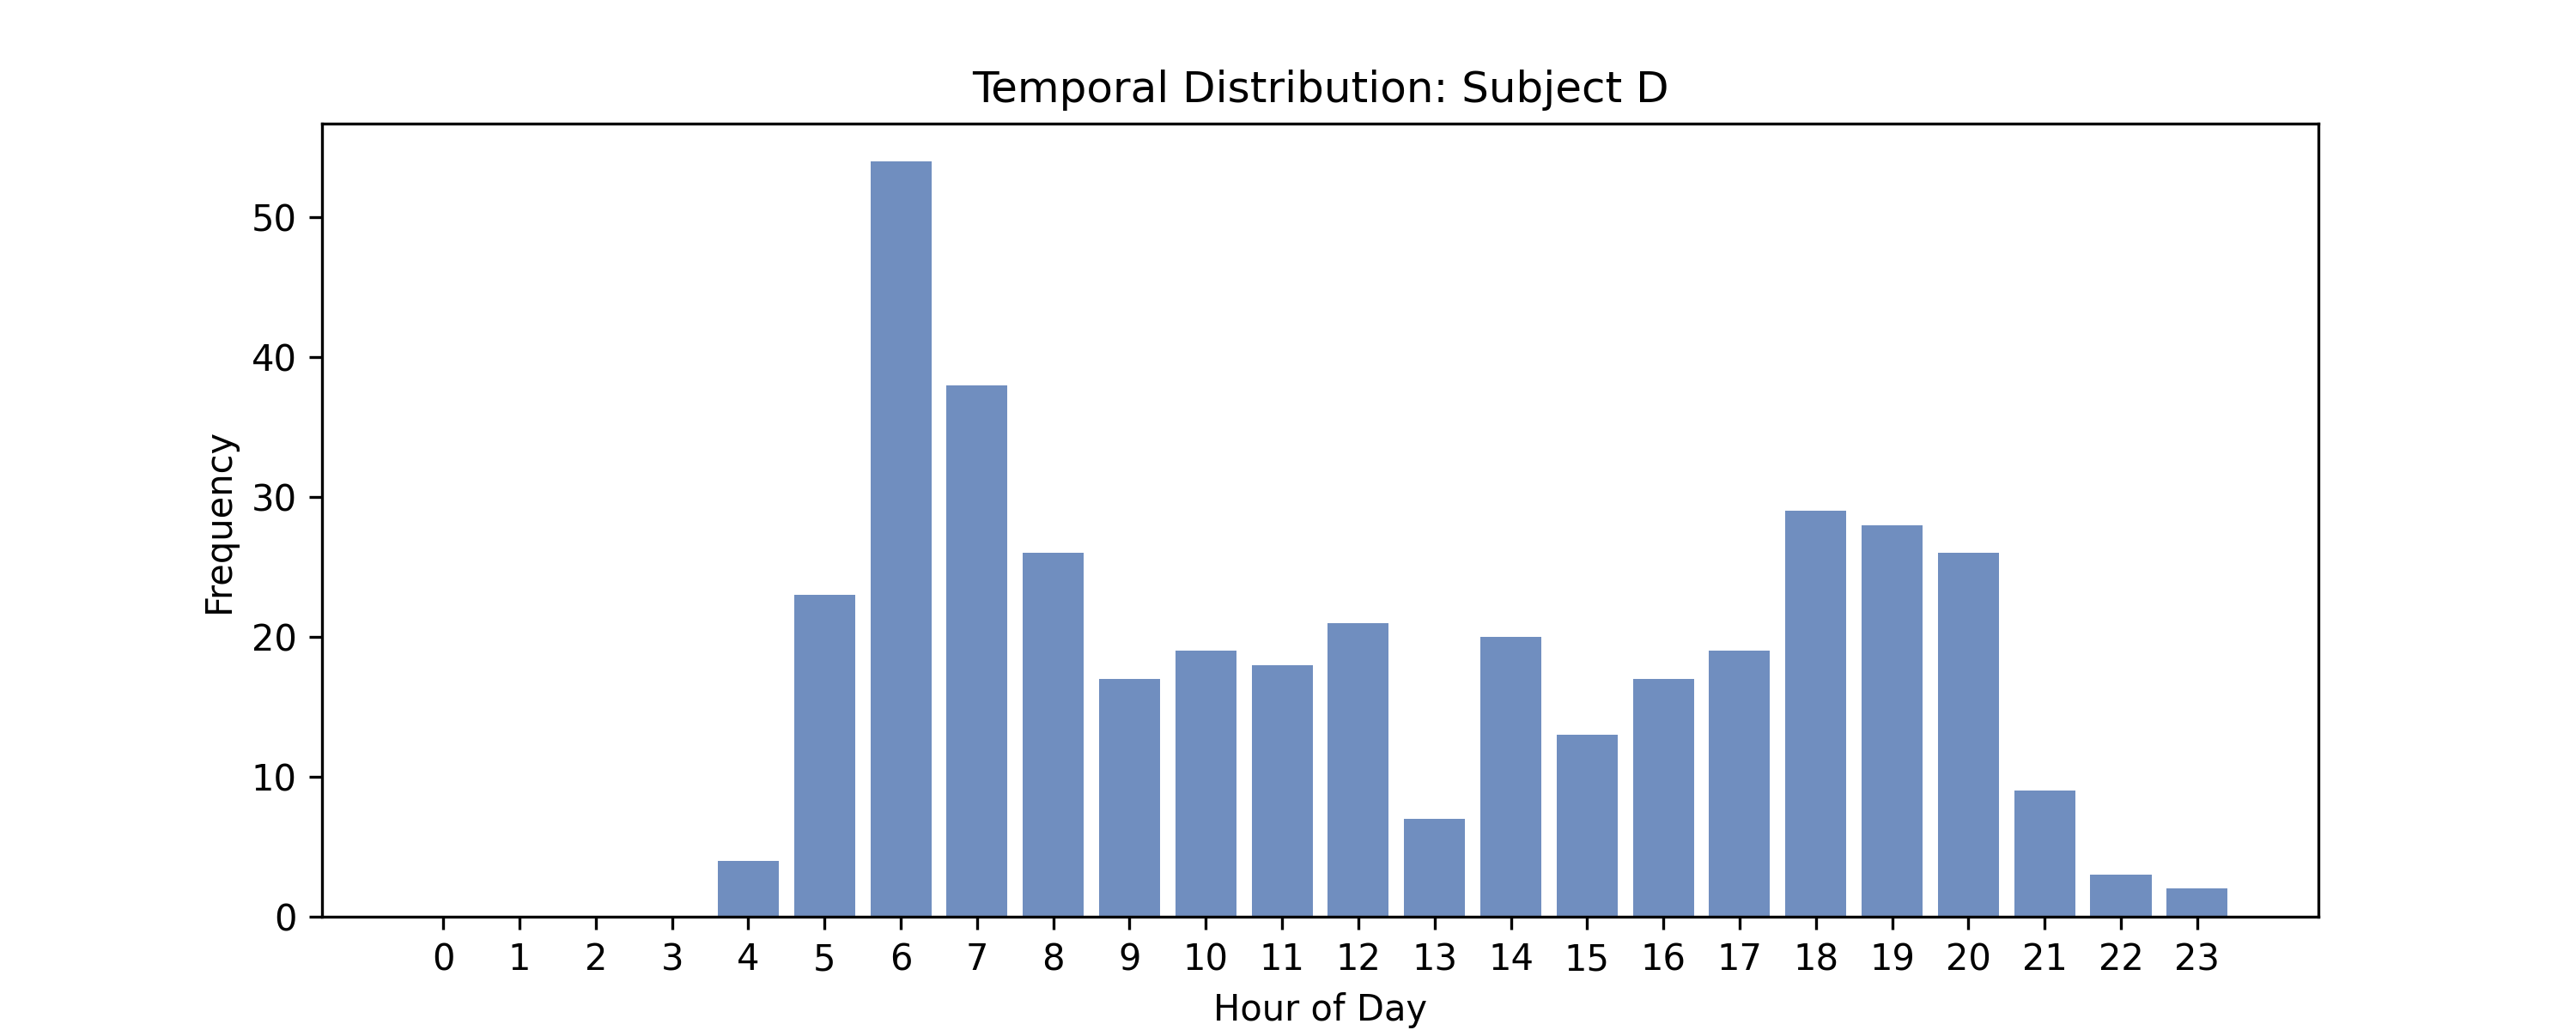
\includegraphics[width=\textwidth]{hourly_Subject_D.png}
		\caption{Subject D}
	\end{subfigure}
	\hfill
	\begin{subfigure}[b]{0.19\textwidth}
		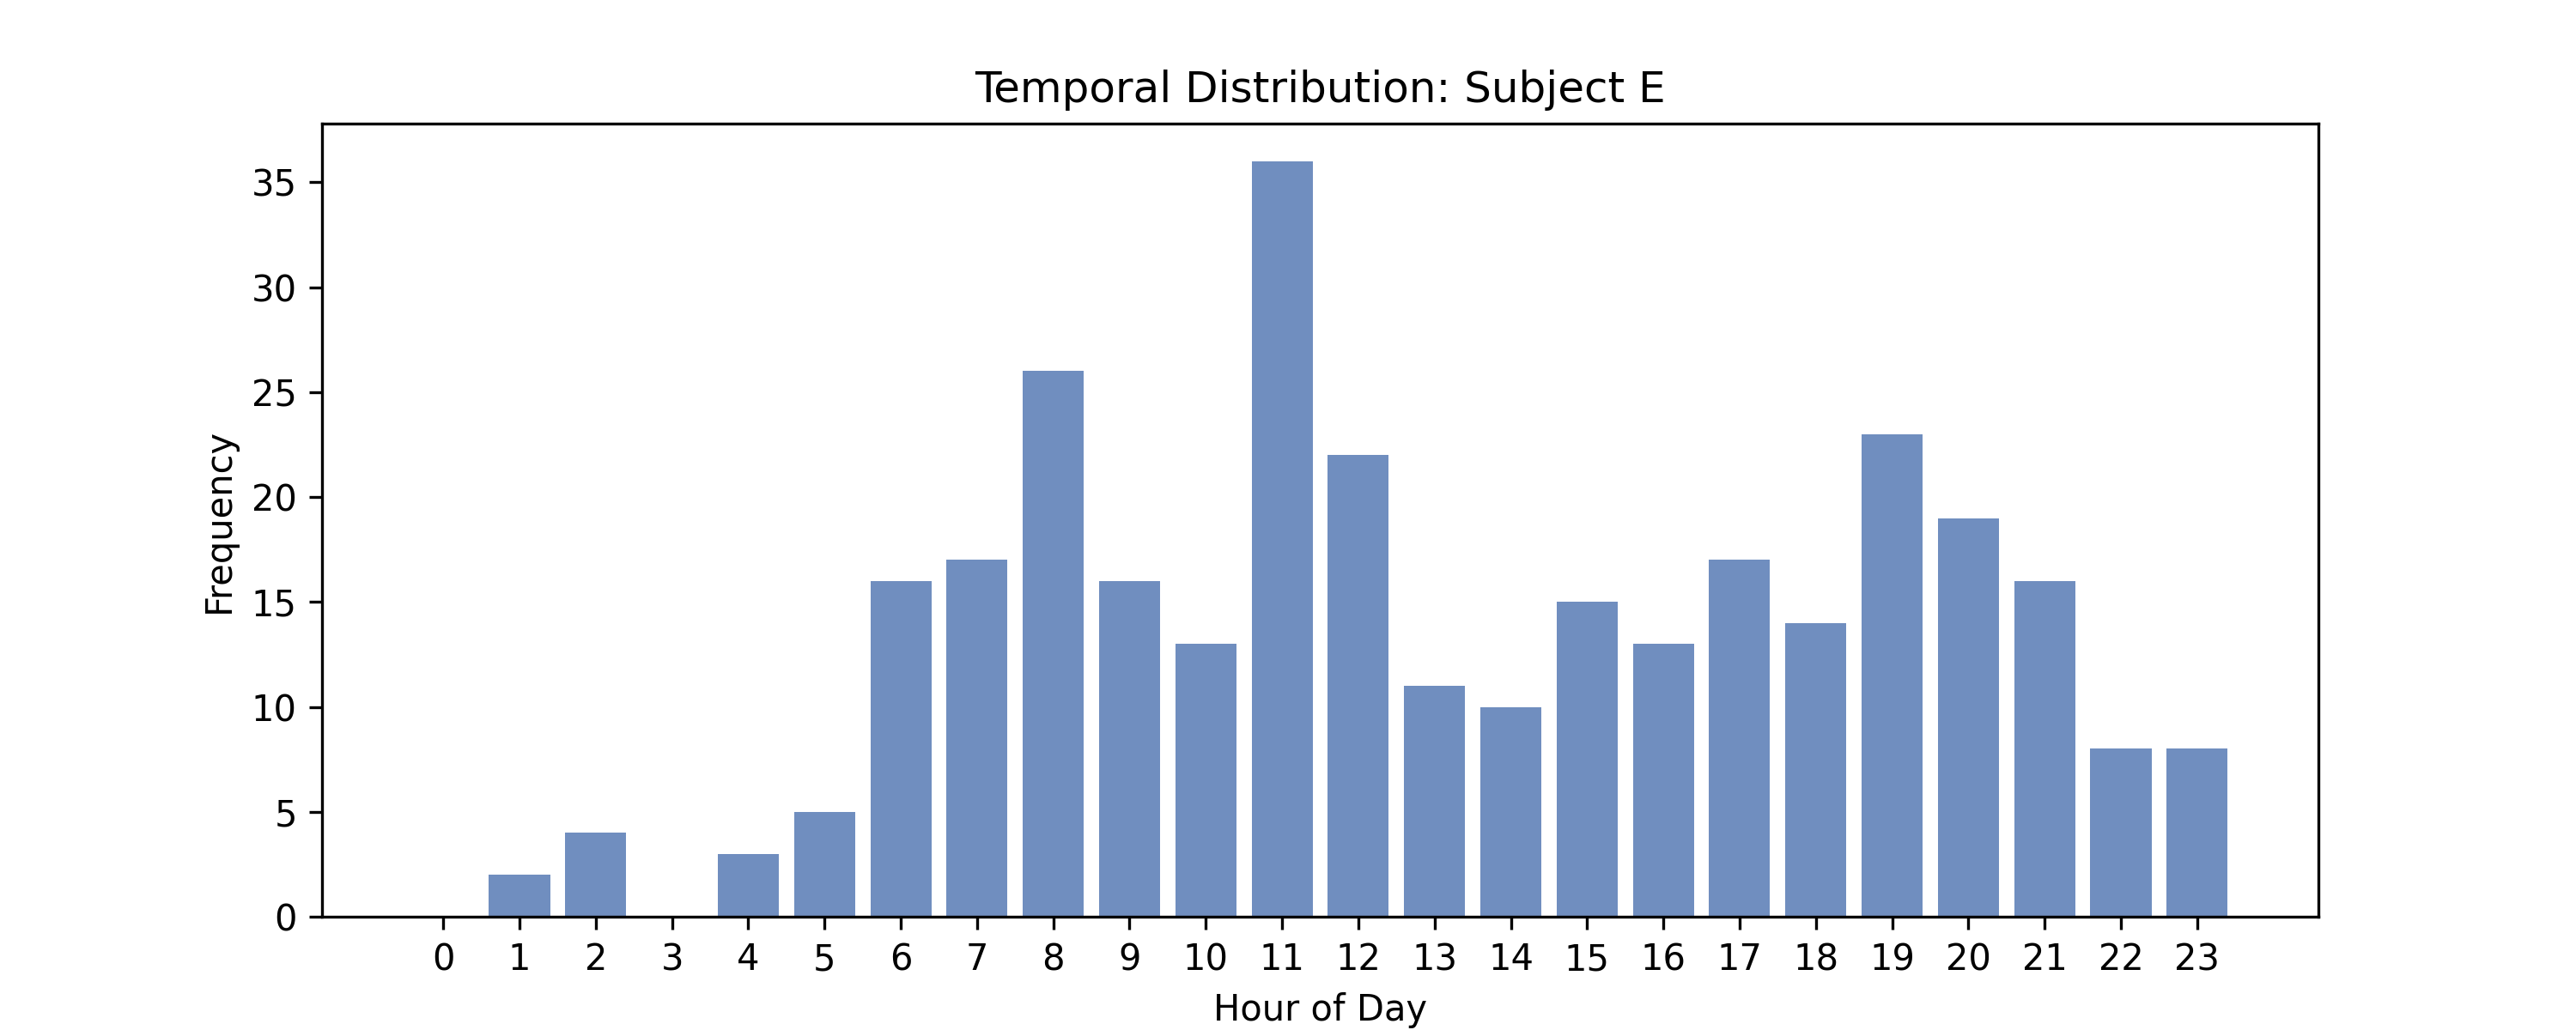
\includegraphics[width=\textwidth]{hourly_Subject_E.png}
		\caption{Subject E}
	\end{subfigure}
	\caption{Hourly frequency of incoming media shares for the top 5 subjects.}
	\label{fig:hourly_all}
\end{figure*}

\subsection{Spatiotemporal and Burst Density Analysis}
To further validate the chronobiological priors, we generated a spatiotemporal heatmap mapping the aggregate high-probability events across the hour of the day and the day of the week (Figure \ref{fig:heatmap}).

\begin{figure}[h!]
	\centering
	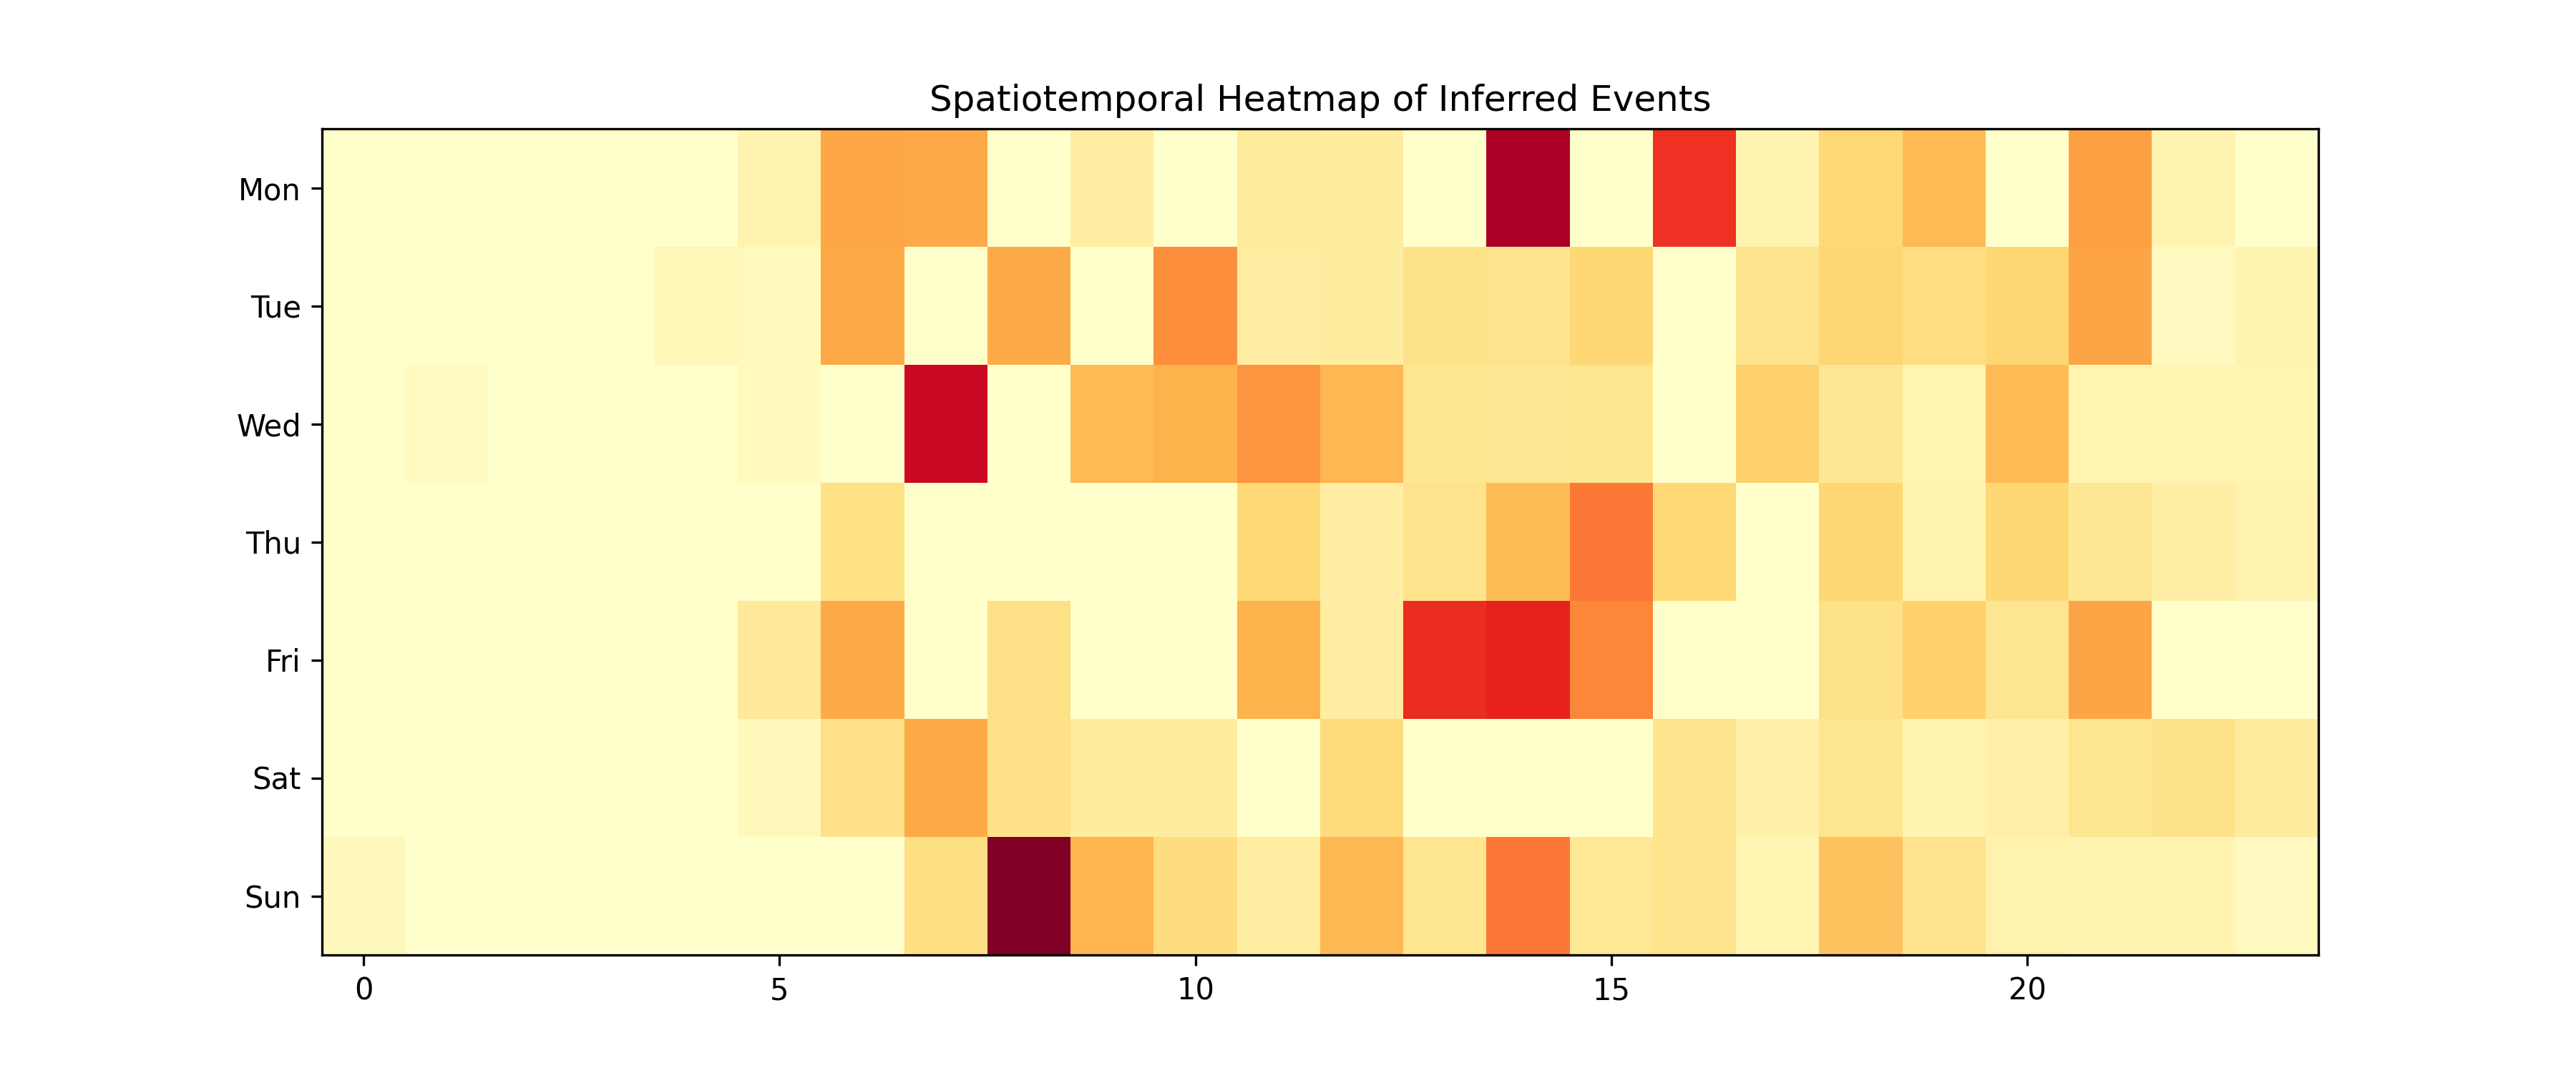
\includegraphics[width=\columnwidth]{heatmap_dow_hour.png}
	\caption{Spatiotemporal heatmap of inferred events. The color intensity represents the aggregate probability score, highlighting weekday vs. weekend circadian shifts.}
	\label{fig:heatmap}
\end{figure}

Furthermore, analyzing the topography of these bursts reveals the critical nature of the time dilation window. Figure \ref{fig:bubble} maps the volume of media sent against the total duration of the burst.

\begin{figure}[h!]
	\centering
	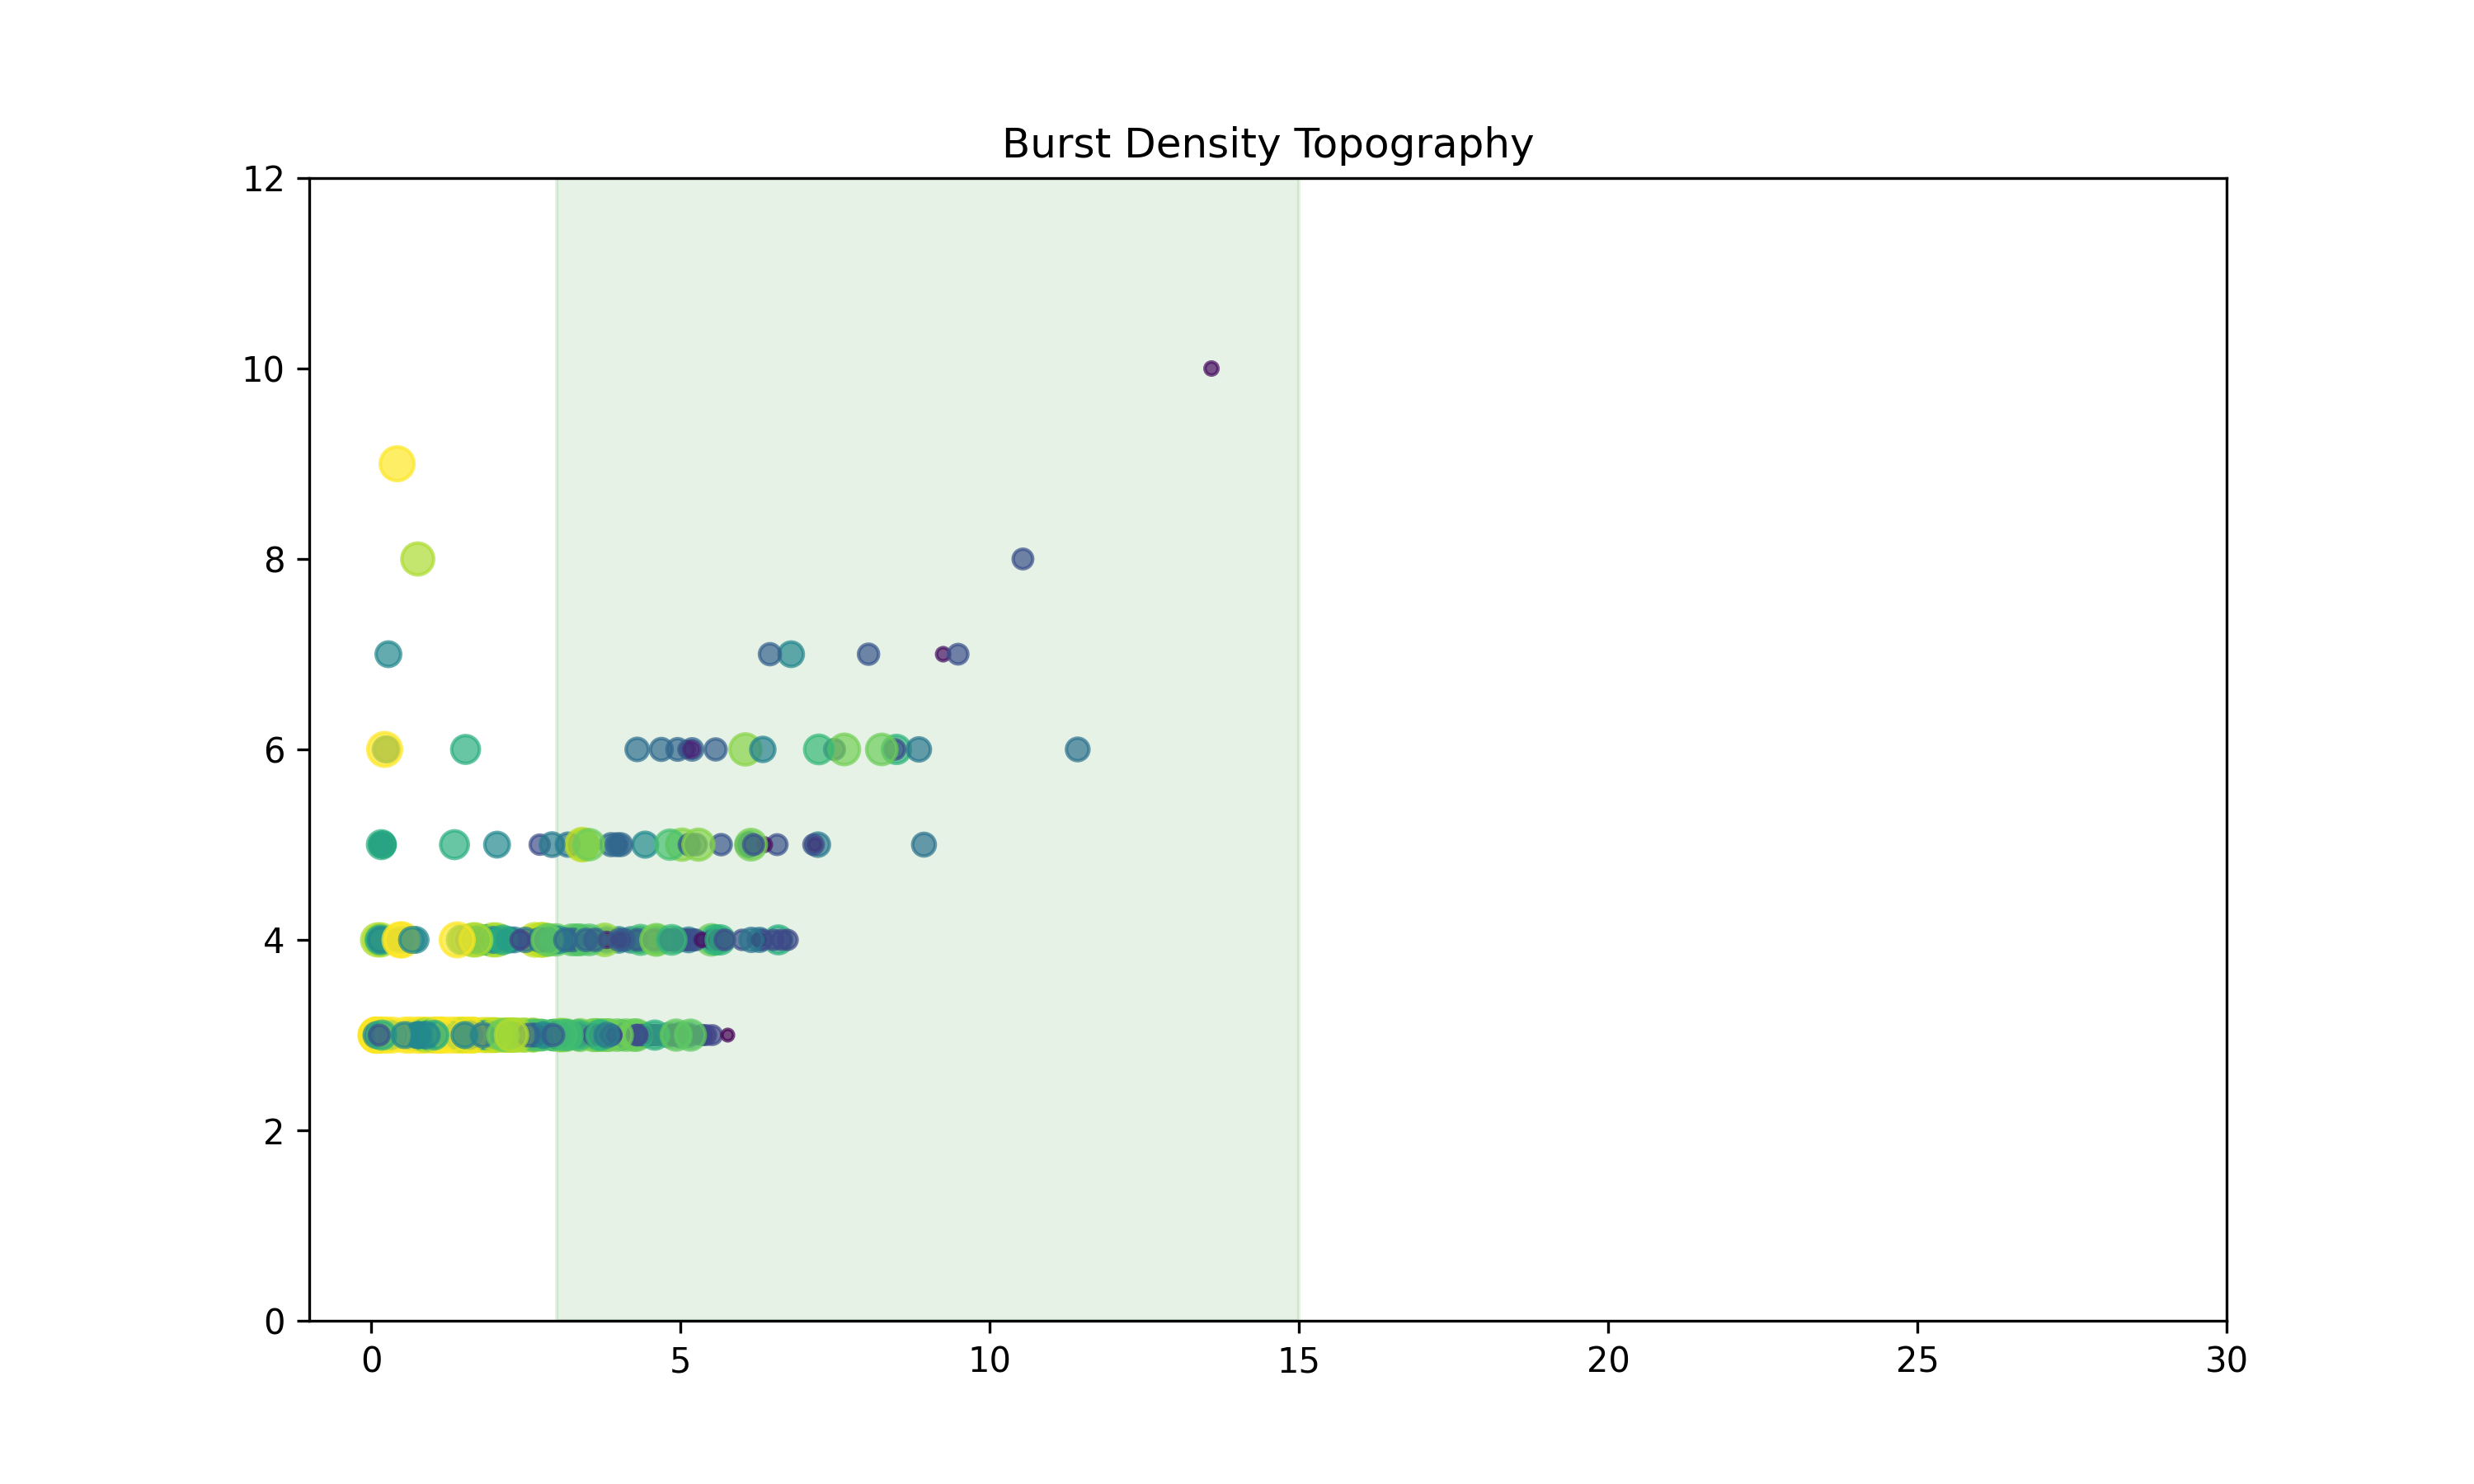
\includegraphics[width=\columnwidth]{burst_density_bubble.png}
	\caption{Burst Density Topography. The shaded region denotes the target temporal dilation window. Bubble size and color correlate with the final inference probability score.}
	\label{fig:bubble}
\end{figure}

\subsection{Inference Timelines}
Upon synthesizing density metrics with the temporal priors, the algorithm outputs discrete inference events. As illustrated in Figure \ref{fig:timelines_all}, we successfully reconstructed prolonged gastrointestinal activity timelines for the top subjects.

\begin{figure*}[h!]
	\centering
	\begin{subfigure}[b]{0.48\textwidth}
		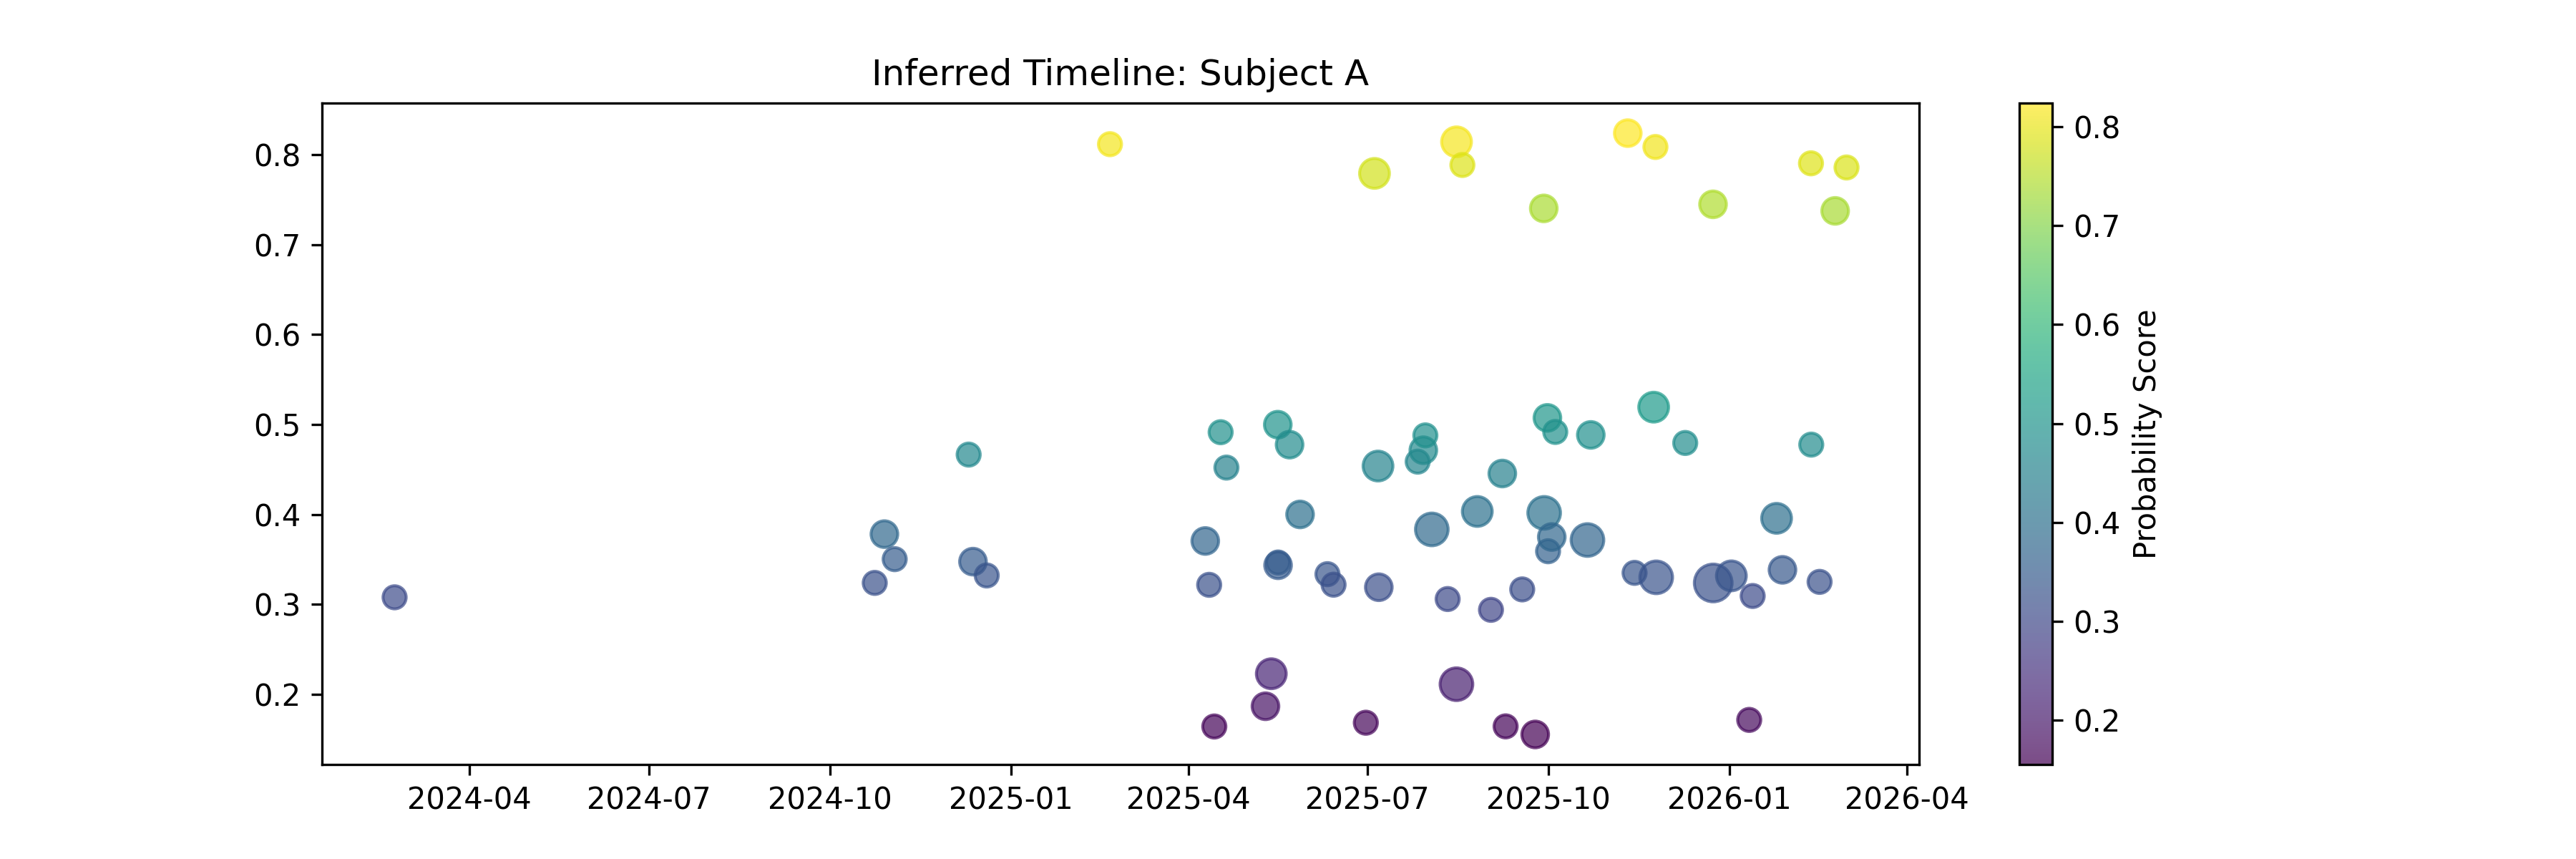
\includegraphics[width=\textwidth]{timeline_Subject_A.png}
		\caption{Subject A}
	\end{subfigure}
	\hfill
	\begin{subfigure}[b]{0.48\textwidth}
		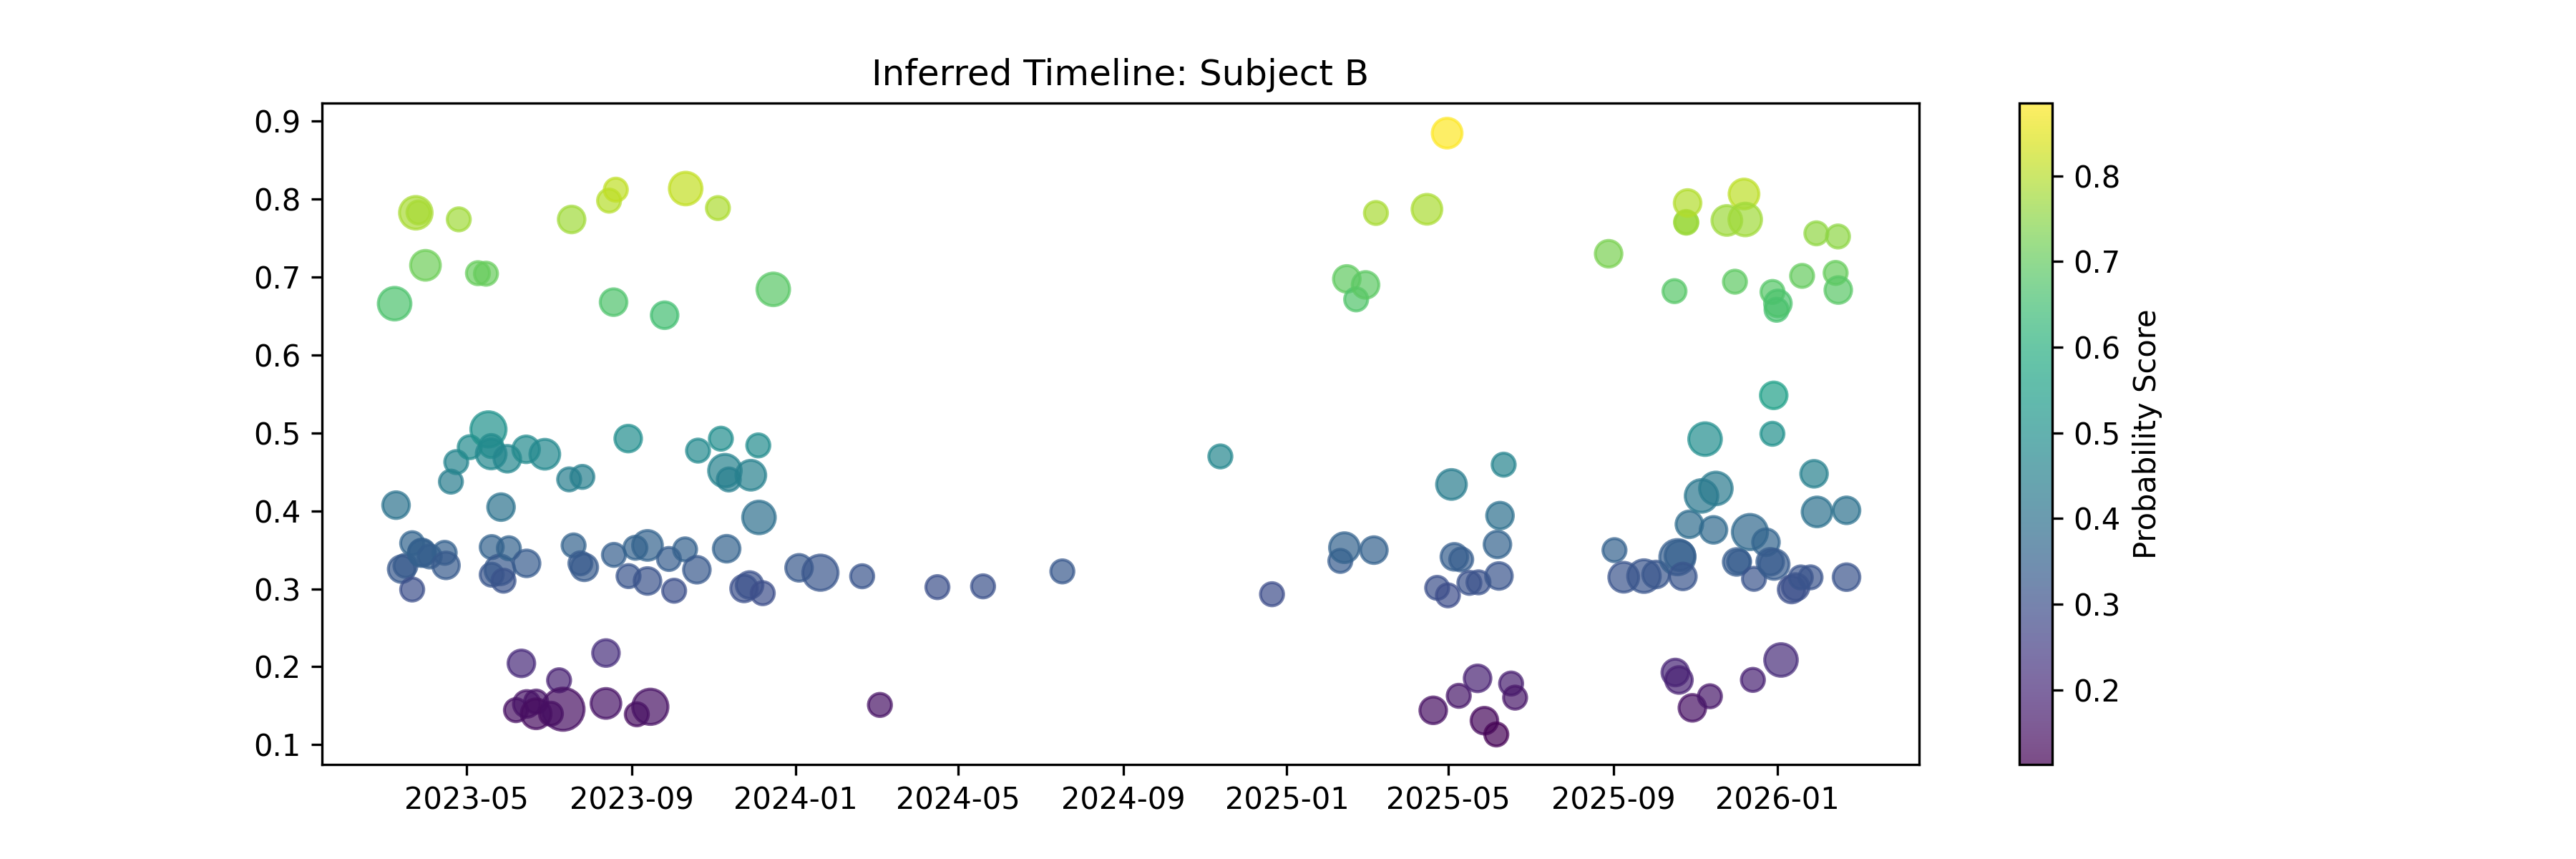
\includegraphics[width=\textwidth]{timeline_Subject_B.png}
		\caption{Subject B}
	\end{subfigure}
	\\
	\begin{subfigure}[b]{0.48\textwidth}
		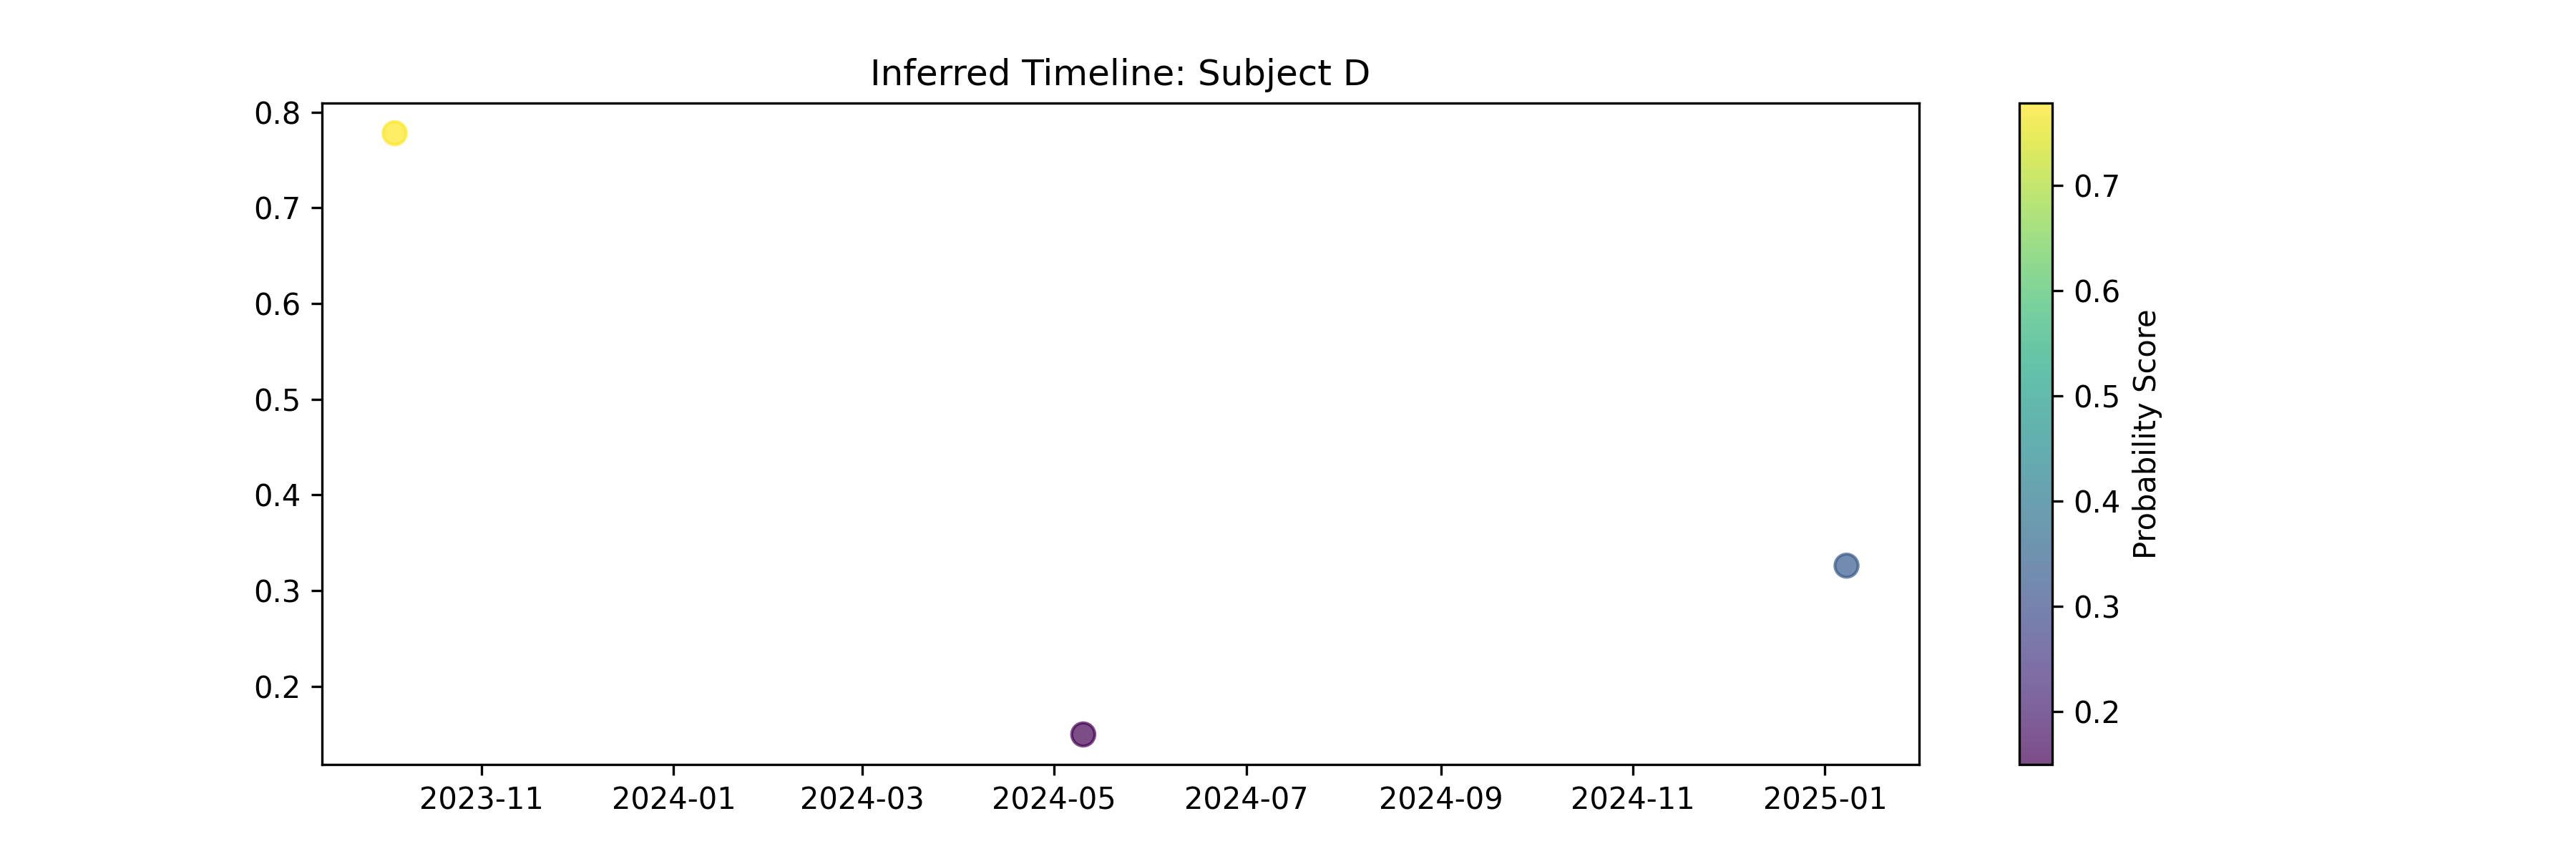
\includegraphics[width=\textwidth]{timeline_Subject_D.png}
		\caption{Subject D}
	\end{subfigure}
	\hfill
	\begin{subfigure}[b]{0.48\textwidth}
		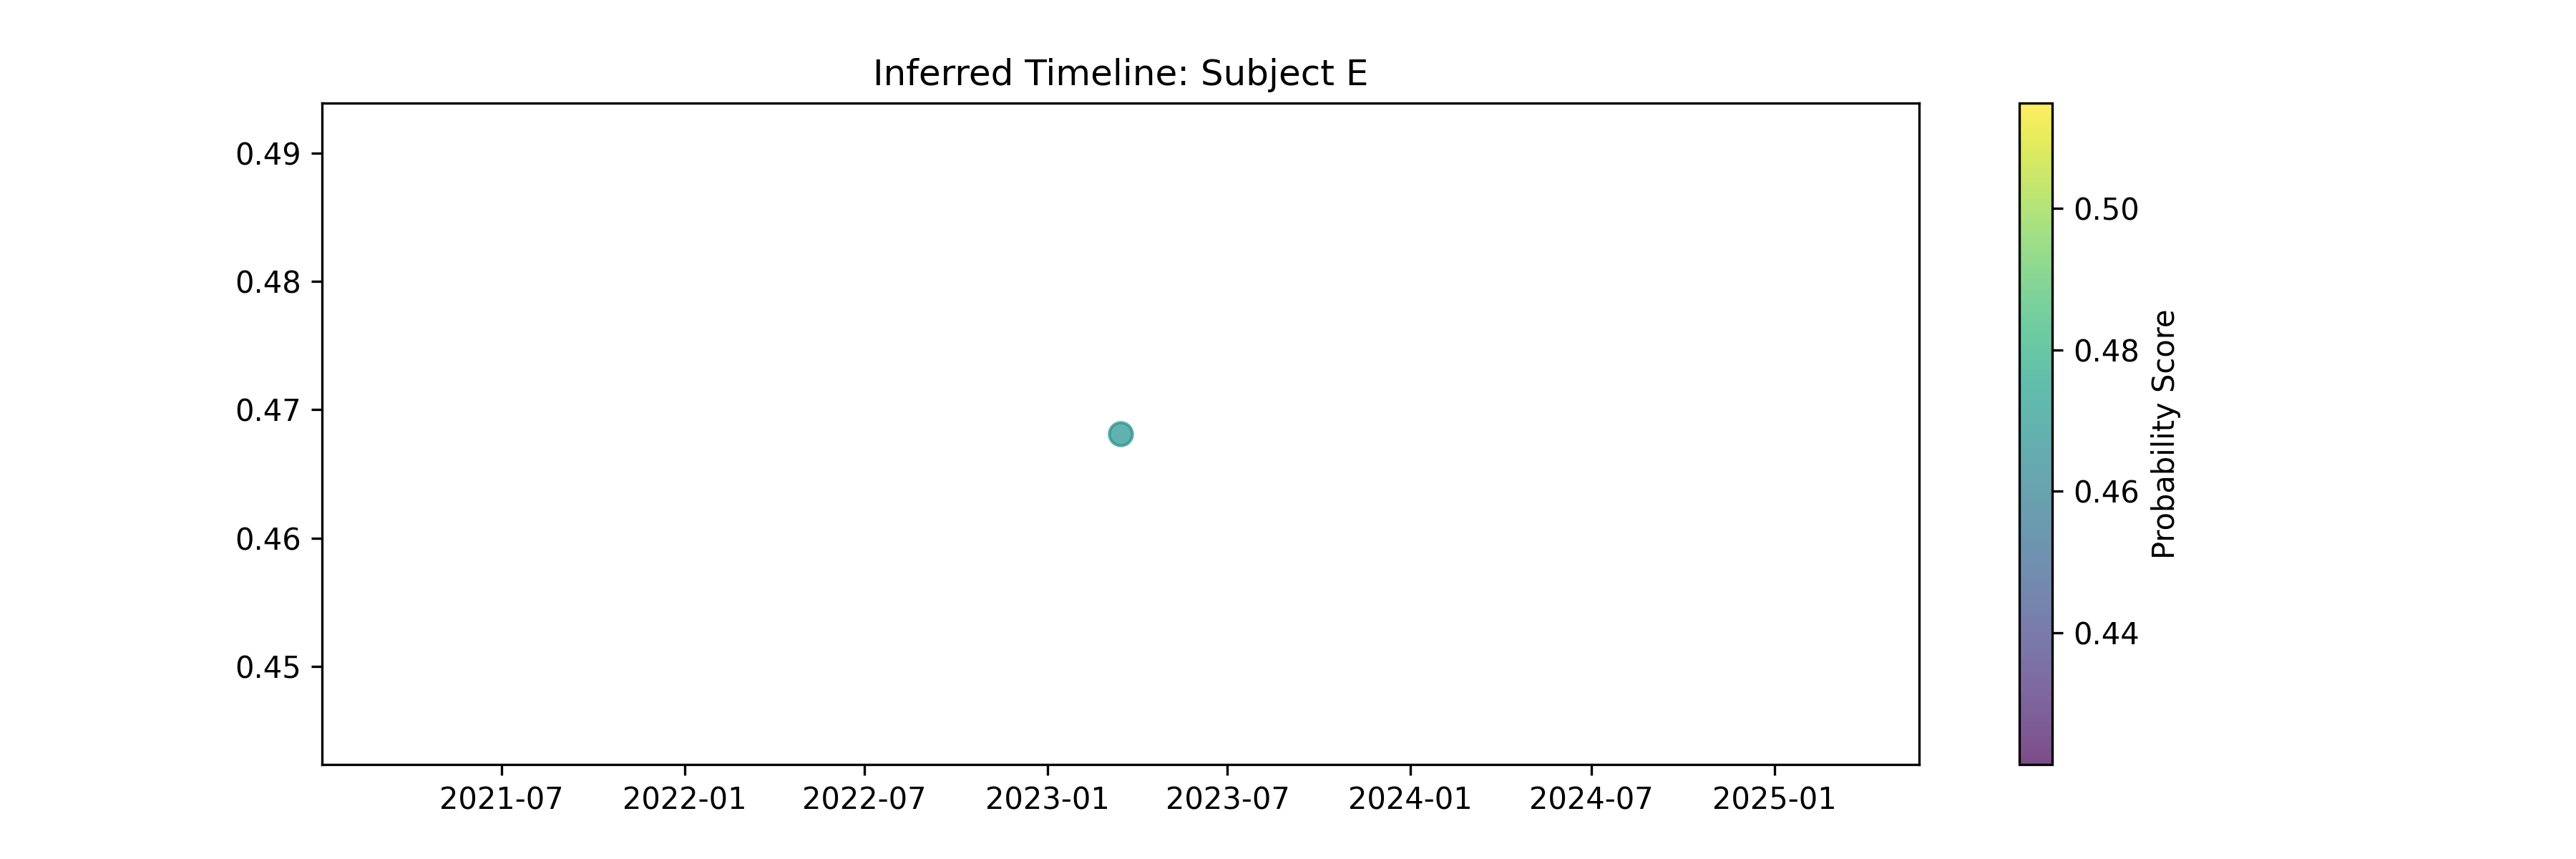
\includegraphics[width=\textwidth]{timeline_Subject_E.png}
		\caption{Subject E}
	\end{subfigure}
	\caption{Inferred bathroom visit timelines for active subjects. Subject C is omitted due to a lack of high-probability clusters meeting the 3--15 minute criteria.}
	\label{fig:timelines_all}
\end{figure*}

\section{Aggregate Global Analysis}
To assess the generalizability of the model, we extended the analysis to the complete archive of 14,708 inbound media shares from 171 unique social peers.

\begin{figure}[h!]
	\centering
	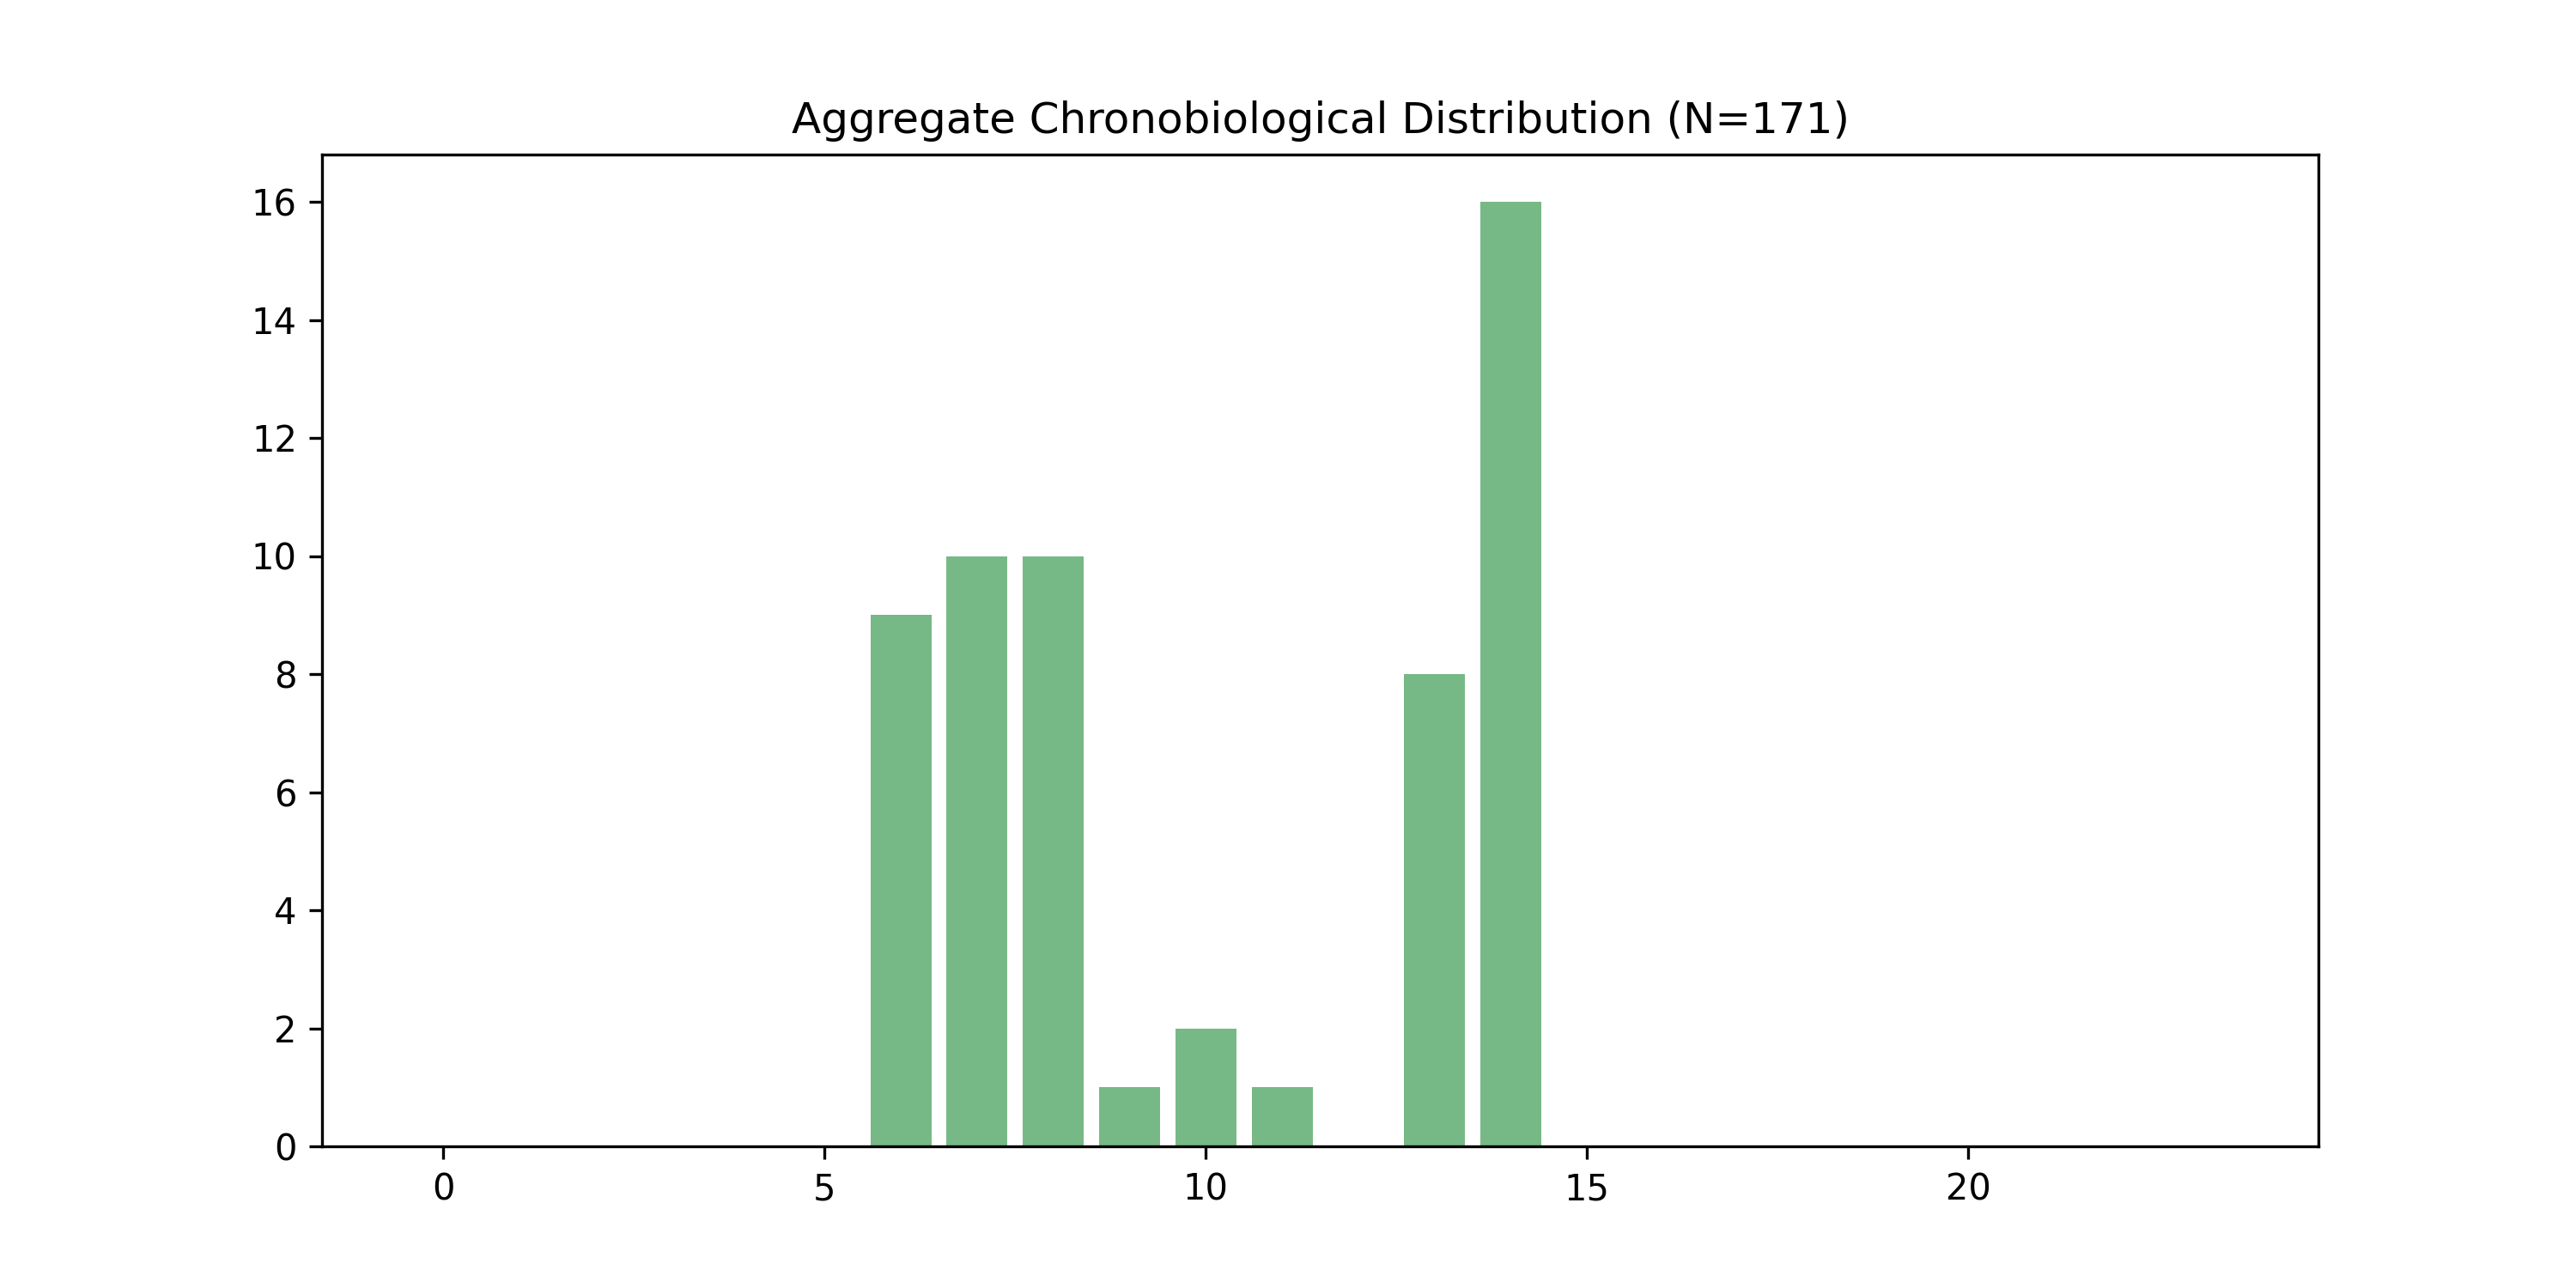
\includegraphics[width=\columnwidth]{global_hourly_distribution.png}
	\caption{Aggregate chronobiological distribution of inferred bathroom visits across 171 unique senders. Note the pronounced early-morning peak.}
	\label{fig:global_hourly}
\end{figure}

The aggregate temporal distribution (Figure \ref{fig:global_hourly}) provides strong empirical evidence for the morning colonic motility surge. The distribution of inference confidence scores (Figure \ref{fig:confidence}) demonstrates the subset of high-probability events.

\begin{figure}[h!]
	\centering
	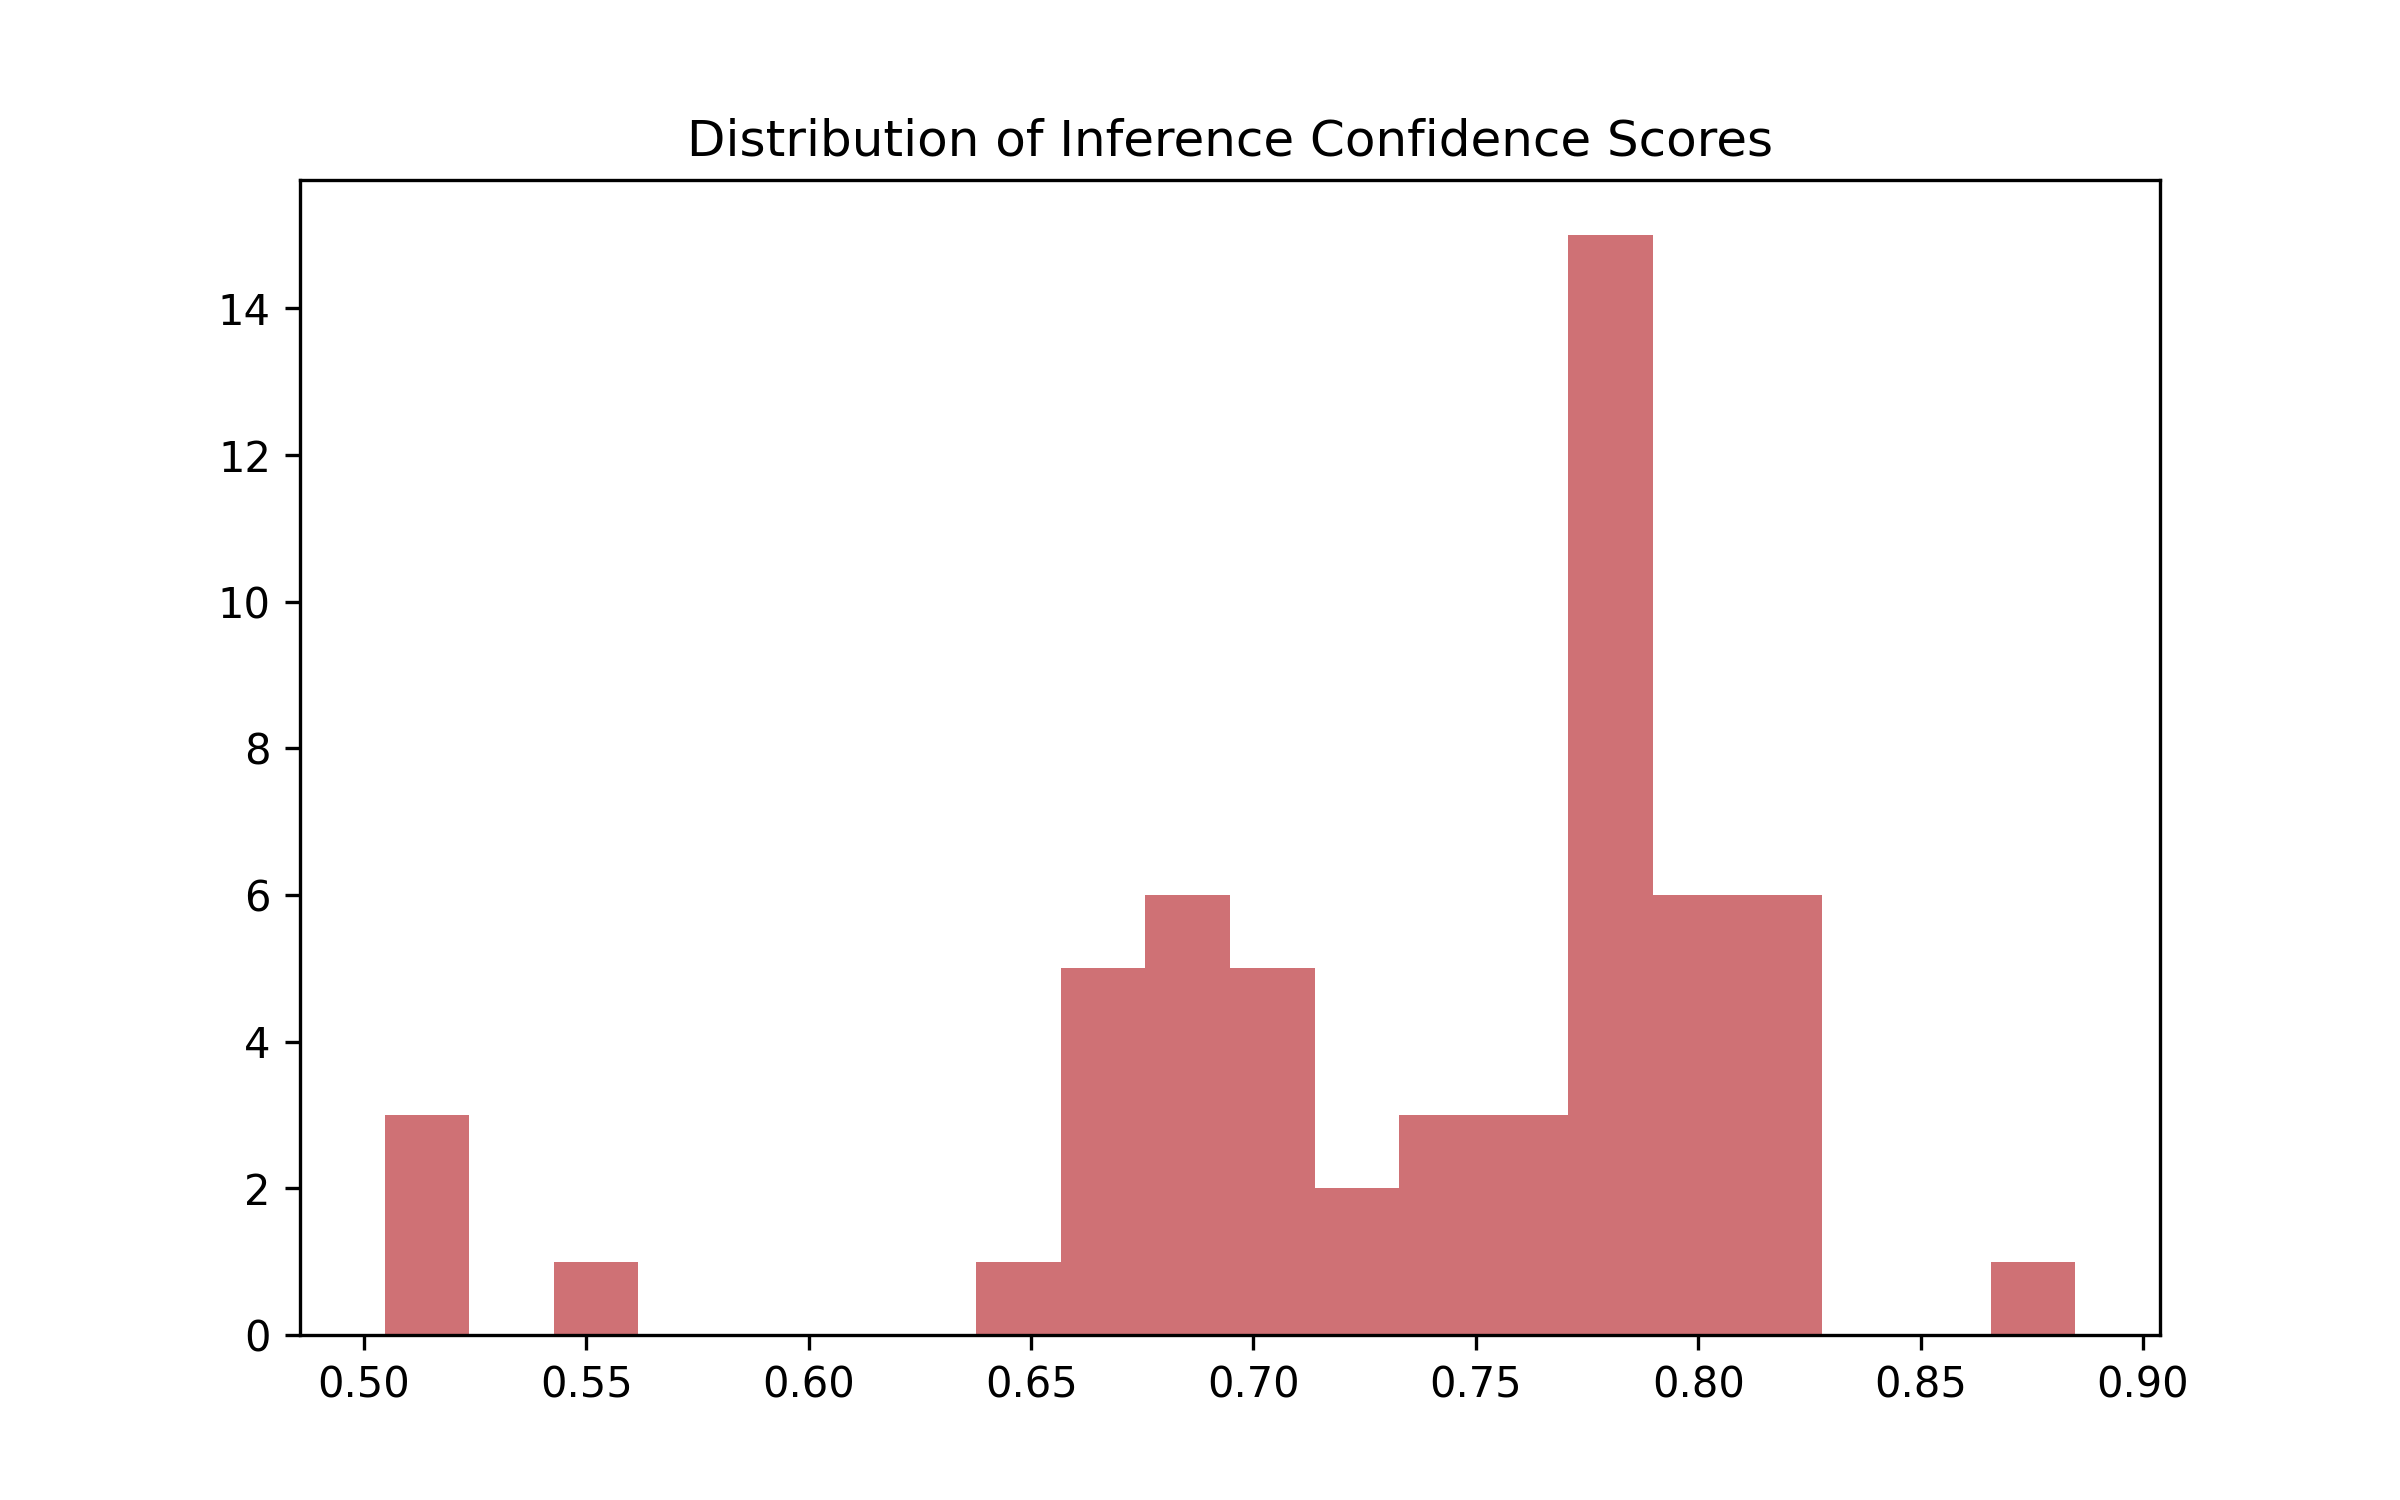
\includegraphics[width=\columnwidth]{inference_confidence_dist.png}
	\caption{Distribution of inference confidence scores for detected temporal bursts across the entire global dataset.}
	\label{fig:confidence}
\end{figure}

\section{Limitations and Future Work}
While the presented methodology demonstrates a novel application of digital phenotyping, several critical limitations must be acknowledged. 

First and foremost is the lack of ground-truth validation. The proposed "Bathroom Events" are defined entirely through mathematical inference based on temporal clustering and chronobiological probabilities. The current study did not utilize patient diaries or physical sensors to verify predictions. To robustly validate this probabilistic model, future researchers should cross-reference the inferred timestamp data against highly invasive empirical measurements, such as deploying acoustic IoT smart-toilet sensors or utilizing smartwatch accelerometer data to detect the distinct physiological signs of the Valsalva maneuver (straining).

Secondly, while the data volume is substantial, the study is limited to the perspective of a single recipient. Larger, multi-recipient cohort studies are required to confirm if these findings are universal.

Finally, the model remains vulnerable to unaddressed confounding variables. A 3--15 minute burst of media sharing during the morning motility peak could be generated by other routine activities such as scrolling on a morning commute or sitting at the breakfast table. Future iterations should seek to integrate secondary data streams, such as device accelerometer data, to disambiguate periods of transit from periods of stasis.

\section{Conclusion}
This research demonstrates that the asynchronous delivery of short-form media acts as a highly accurate telemetry system for human gastrointestinal activity. By synthesizing multi-disciplinary streams, ranging from chronobiology to heavy-tailed human communication dynamics, we have established a robust probabilistic framework for objective digital phenotyping. Ultimately, this work proves that even the most private biological functions leave a discernible footprint in the modern digital ether.

\begin{thebibliography}{9}
	\bibitem{jayakumar2020}
	Jayakumar P, Lin E, Galea V, et al. Digital Phenotyping and Patient-Generated Health Data for Outcome Measurement in Surgical Care: A Scoping Review. \textit{J Pers Med}. 2020;10(4):282. Published 2020 Dec 15. doi:10.3390/jpm10040282.
	
	\bibitem{ramprasad2025}
	Ramprasad C, Wu C, Chang J, et al. Smartphone use on the toilet and the risk of hemorrhoids. \textit{PLoS One}. 2025 Sep 3;20(9):e0329983. doi:10.1371/journal.pone.0329983.
	
	\bibitem{qssupplies}
	QS Supplies. Bathroom Doomscrolling. Available from: \url{https://www.qssupplies.co.uk/bathroom-doomscrolling.html}
	
	\bibitem{hibberd2023}
	Hibberd TJ, Ramsay S, Spencer-Merris P, et al. Circadian rhythms in colonic function. \textit{Front Physiol}. 2023;14:1239278. Published 2023 Aug 30. doi:10.3389/fphys.2023.1239278.
	
	\bibitem{barabasi2005}
	Barabási AL. The origin of bursts and heavy tails in human dynamics. \textit{Nature}. 2005;435(7039):207-211. Center for Complex Networks Research and Department of Physics, University of Notre Dame.
\end{thebibliography}

\end{document}
